\documentclass[cs4size,a4paper]{ctexart}   
%==================== 数学符号公式 ============
\usepackage{amsmath}                 % AMS LaTeX宏包
\usepackage[style=1]{mdframed}
\usepackage{amsthm}
\usepackage{amsfonts}
\usepackage{mathrsfs}                % 英文花体字体
\usepackage{bm}                      % 数学公式中的黑斜体
\usepackage{bbding,manfnt}           % 一些图标,如 \dbend
\usepackage{lettrine}                % 首字下沉,命令\lettrine
\def\attention{\lettrine[lines=2,lraise=0,nindent=0em]{\large\textdbend\hspace{1mm}}{}}
\usepackage{longtable}
\usepackage[toc,page]{appendix}
\usepackage{geometry}                % 页边距调整
\usepackage{makecell}                % 表格内换行
\geometry{top=3.0cm,bottom=2.7cm,left=2.5cm,right=2.5cm}
%====================公式按章编号==========================
\numberwithin{equation}{section}
\numberwithin{table}{section}
\numberwithin{figure}{section}
%================= 基本格式预置 ===========================
\usepackage{fancyhdr}
\pagestyle{fancy}
\fancyhf{}  
\fancyhead[C]{\zihao{5}  \kaishu fancyhead千万别忘改了}
\fancyfoot[C]{~\zihao{5} \thepage~}
\renewcommand{\headrulewidth}{0.65pt} 
% \CTEXsetup[format={\centering\bfseries\zihao{-2}},name={第, 章}]{section}
\CTEXsetup[format={\centering\bfseries\zihao{4}}]{section}
\CTEXsetup[format={\bfseries \zihao{4}}]{subsection}
\CTEXsetup[format={\bfseries \zihao{-4}}]{subsubsection}
%================== 图形支持宏包 =========================
\usepackage{subfig}
\usepackage{graphicx}                % 嵌入png图像
\usepackage{color,xcolor}            % 支持彩色文本、底色、文本框等
\usepackage{hyperref}                % 交叉引用
\usepackage{caption}
\captionsetup{figurewithin=section}
%==================== 源码和流程图 =====================
\usepackage{listings}                % 粘贴源代码
\usepackage{xcolor}

\lstset{
	numbers=left, % 显示行号
	numberstyle=\tiny, % 行号字体
	keywordstyle=\color{blue!70}, % 关键字颜色
	commentstyle=\color{red!50!green!50!blue!50}, % 注释颜色
	frame=shadowbox, % 为代码块添加阴影框
	rulesepcolor=\color{red!20!green!20!blue!20}, % 阴影框颜色
	escapeinside=``, % 允许在代码块中使用 LaTeX 命令
	xleftmargin=1em, xrightmargin=1em, aboveskip=1em, % 设置代码块的边距
	framexleftmargin=2em % 阴影框左边距
} 


\usepackage{color}
\definecolor{dkgreen}{rgb}{0,0.6,0}
\definecolor{gray}{rgb}{0.5,0.5,0.5}
\definecolor{mauve}{rgb}{0.58,0,0.82}
 \usepackage{xcolor}

% \renewcommand{\lstlistingname}{代码}    % 代码标题样式修改无效?!
%  \lstset{
%     basicstyle          =   \sffamily,          % 基本代码风格
%     keywordstyle        =   \bfseries,          % 关键字风格
%     commentstyle        =   \rmfamily\itshape,  % 注释的风格,斜体
%     stringstyle         =   \ttfamily,  % 字符串风格
%     flexiblecolumns,                % 别问为什么,加上这个
%     numbers             =   left,   % 行号的位置在左边
%     showspaces          =   false,  % 是否显示空格,显示了有点乱,所以不现实了
%     numberstyle         =   \zihao{5}\ttfamily,    % 行号的样式,小五号,tt等宽字体
%     showstringspaces    =   false,
%     captionpos          =   t,      % 这段代码的名字所呈现的位置,t指的是top上面
%     frame               =   lrtb,   % 显示边框
% }

%  \lstdefinestyle{SPICE}{
%     language        =   matlab, % 语言选Python
%     basicstyle      =   \zihao{-5}\ttfamily,
%     numberstyle     =   \zihao{-5}\ttfamily,
%     keywordstyle    =   \color{blue},
%     keywordstyle    =   [2] \color{teal},
%     stringstyle     =   \color{magenta},
%     commentstyle    =   \color{red}\ttfamily,
%     breaklines      =   true,   % 自动换行,建议不要写太长的行
%     columns         =   fixed,  % 如果不加这一句,字间距就不固定,很丑,必须加
%     basewidth       =   0.5em,
% }

%--------------------
\hypersetup{hidelinks}
\usepackage{booktabs}  
\usepackage{shorttoc}
\usepackage{tabu,tikz}
\usepackage{float}

\usepackage{multirow}



\tabcolsep=1ex
\tabulinesep=\tabcolsep
\newlength\tikzboxwidth
\newlength\tikzboxheight
\newcommand\tikzbox[1]{%
        \settowidth\tikzboxwidth{#1}%
        \settoheight\tikzboxheight{#1}%
        \begin{tikzpicture}
        \path[use as bounding box]
                (-0.5\tikzboxwidth,-0.5\tikzboxheight)rectangle
                (0.5\tikzboxwidth,0.5\tikzboxheight);
        \node[inner sep=\tabcolsep+0.5\arrayrulewidth,line width=0.5mm,draw=black]
                at(0,0){#1};
        \end{tikzpicture}%
        }

\makeatletter
\def\hlinew#1{%
  \noalign{\ifnum0=`}\fi\hrule \@height #1 \futurelet
   \reserved@a\@xhline}
   
\newcommand{\tabincell}[2]{\begin{tabular}{@{}#1@{}}#2\end{tabular}}%

\usepackage{subfig}

\usepackage{CJK}
\usepackage{ifthen}


\usepackage{graphicx} 
\newcommand{\HRule}{\rule{\linewidth}{0.5mm}}

\newtheorem{Theorem}{定理}
\newtheorem{Lemma}{引理} 
%%使得公式随章节自动编号
\makeatletter
\@addtoreset{equation}{section}
\makeatother
\renewcommand{\theequation}{\arabic{section}.\arabic{equation}}

%-------------------------
	
\usepackage{pythonhighlight}
\usepackage{tikz}                    
\usepackage{tikz-3dplot}
\usetikzlibrary{shapes,arrows,positioning}
%===================   正文开始    ===================
\begin{document}
\bibliographystyle{gbt7714-2005}     %论文引用格式
%===================  定理类环境定义 ===================
\newtheorem{example}{例}              % 整体编号
\newtheorem{algorithm}{算法}
\newtheorem{theorem}{定理}            % 按 section 编号
\newtheorem{definition}{定义}
\newtheorem{axiom}{公理}
\newtheorem{property}{性质}
\newtheorem{proposition}{命题}
\newtheorem{lemma}{引理}
\newtheorem{corollary}{推论}
\newtheorem{remark}{注解}
\newtheorem{condition}{条件}
\newtheorem{conclusion}{结论}
\newtheorem{assumption}{假设}
%==================重定义 ===================
\renewcommand{\contentsname}{目录}     
\renewcommand{\abstractname}{摘要} 
\renewcommand{\refname}{参考文献}     
\renewcommand{\indexname}{索引}
\renewcommand{\figurename}{图}
\renewcommand{\tablename}{表}
\renewcommand{\appendixname}{附录}
\renewcommand{\proofname}{证明}
\renewcommand{\algorithm}{算法} 
%============== 封皮和前言 =================
% \input{body/cover}
\pagestyle{plain}
\pagenumbering{arabic}
% \include{body/abstract}
\pagestyle{empty}
% \tableofcontents 
% \thispagestyle{empty}
%============== 论文正文   =================
% \pagestyle{fancy}
\pagestyle{plain}
% \include{body/chapter1}      %
% \include{body/chapter2}
% \include{body/chapter3}
% \include{body/chapter4}
% \include{body/chapter5}
% \include{body/chapter6}

\begin{center}
    \textsc{\zihao{3} \bfseries ADDA课程项目}\\[0.3cm]
\end{center}

\begin{center}
	组员:冯俊杰、贾梓越、陈江华、陈畅
\end{center}

\newpage
\tableofcontents

\newpage
\section{设计目标}
\noindent
研究内容:

通过 matlab 建模或者 cadence(MOS 管级/verilogA 级,工艺不限)构建一个时钟交
织 Pipelined-SAR ADC,pipelined 级数不限,时钟校准通道数≥4 条,精度≥12 位,
TI-ADC 总采样率≥2GS/s,自己手动添加以下误差和失配,例如采样时钟 jitter 范围
100fs~5ps,timing skew 范围 200fs~5ps, inter-stage gain error± 10%等(以上参
数仅供参考), 通过静态分析方法和动态分析方法分析:TI mismatch (gain mismatch,
offset mismatch and timing skew), pipelined-SAR ADC 级间增益误差(inter-stage 
gain error), 第一级 SAR ADC 电容失配(capacitor-DAC mismatch),比较器失调,
时钟 jitter 等的影响。选择一种 time skew 校准方法进行 timing skew 误差检测并分
析。建模、仿真验证、撰写完整分析报告,在 cadence 里面完成仿真验证的有额外 bonus
分数。

\noindent
分析方法:

静态特性分析:转移特性曲线/统计方法;动态特性分析:FFT

\noindent
最终实现:

用matlab构建了一个理想精度为15bit的四通道时钟交织两级流水SAR ADC。并自行引入了时钟抖动、时序偏差、增益误差等影响因素,并通过静态分析方法和动态分析方法分析了其对ADC性能的影响。最后对timing skew进行了校准。

\newpage
\section{电路结构及原理}

    \subsection{Pipeline SAR ADC建模原理}
        基本架构:如图\ref{fig:circuit1}所示,两级SAR级间插入一个余量放大器。
        	\begin{figure}[H]
        		\centering
        		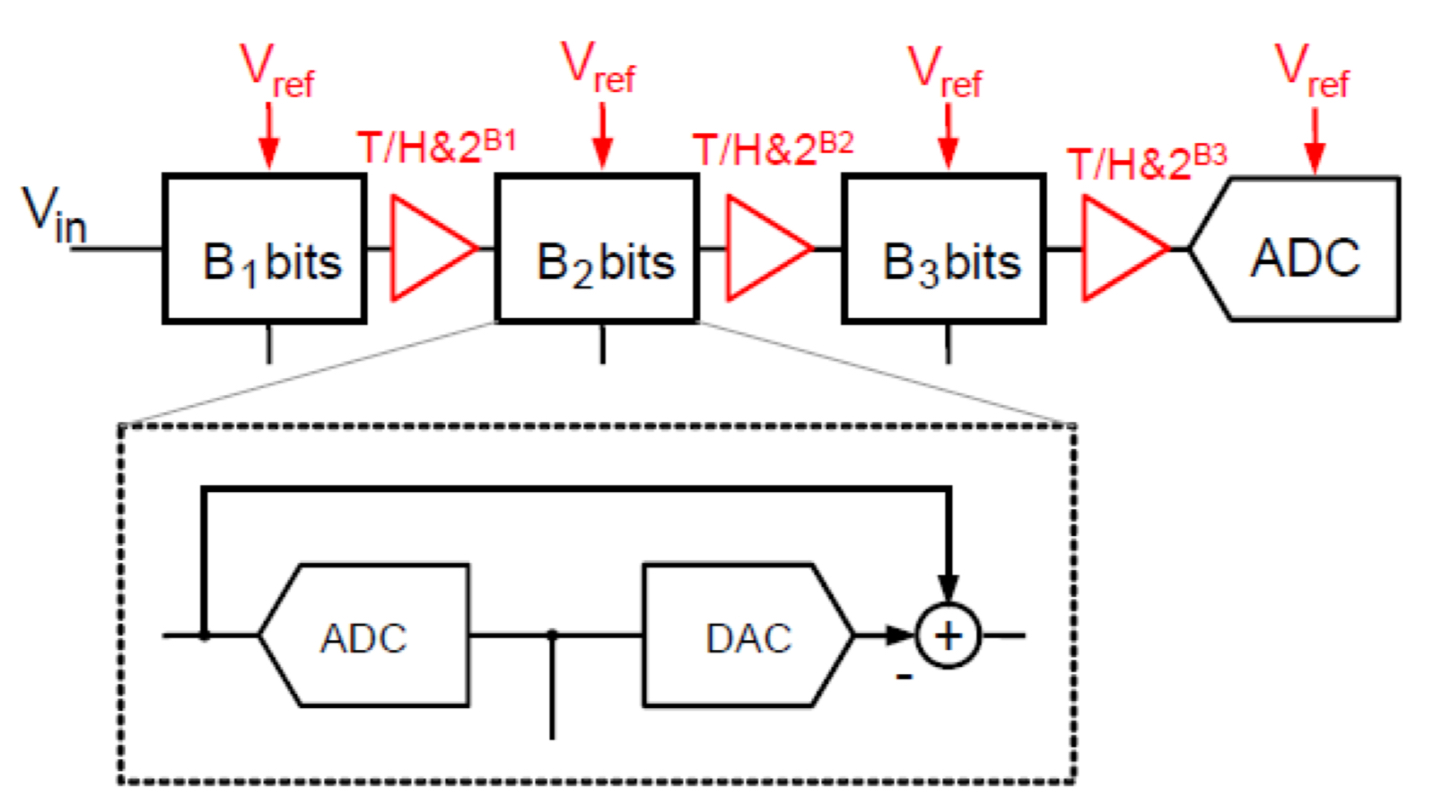
\includegraphics[width=0.5\textwidth]{figure/circuit1.jpg}
        		\caption{pipeline级联原理图} \label{fig:circuit1}
        	\end{figure}
        	
        总位数为
            \begin{equation}
                N=N_1+N_2+...-R
            \end{equation}
            
        N为总位数,其中R为冗余位。
        
        \textbf{\textit{在设计时需要注意以下几点:}}
        \begin{itemize}
			\item \textbf{时序设计基本原则:}$fs=1/Ts$,其中$Ts = min\{Ts_1,Ts_2,...\}$,由于采样率取决于最慢的周期,设计时尽量让每级周期近似相等,避免时序浪费。
			\item \textbf{余量传输:}如图\ref{fig:circuit2}所示,正常需要将数字量经过DAC转回模拟域,但考虑SAR采用电容开关阵列,可以加一位电容,利用SAR本身开关阵列实现DAC,得到余差。即纯SAR ADC的开关阵列正常需要N-2位电容,但若要利用电容开关阵列实现DAC功能,应当考虑N-1位电容,这就造成了前后级的结构不同,因为最后一级只需实现纯SAR ADC,无需再转换回模拟域。
				\begin{figure}[H]
					\centering
					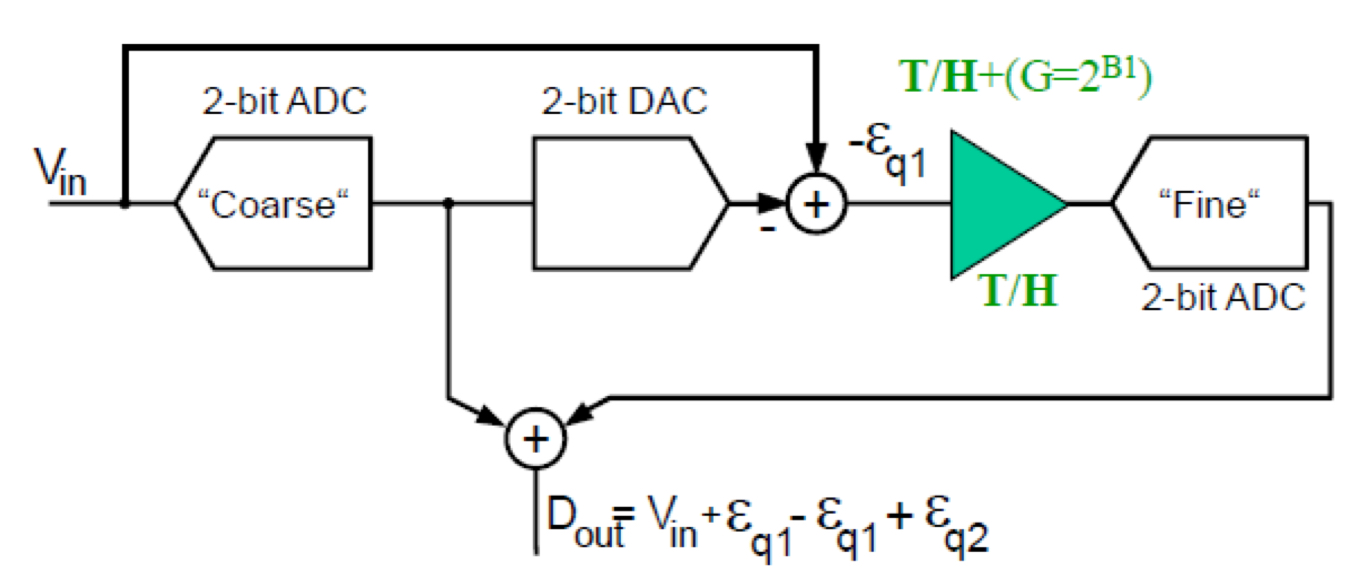
\includegraphics[width=0.7\textwidth]{figure/circuit2.jpg}
					\caption{余量放大传输原理图} \label{fig:circuit2}
				\end{figure}
			以2级流水线为例,若第一级M1位,第二级M2位,则实际第一级的ADC需要M1-1位电容,而第二即只需要M2-2位电容。
			\item \textbf{放大倍数:}
				\begin{equation}
					G=2^{M1-R-K}=2^{M1-R}\cdot\frac{Vref2}{Vref1}
				\end{equation}
			M1为前级ADC的位数。
			
			R为冗余位的位数——引入冗余的目的是为了采用冗余位校正算法来校正比较器失调和DAC建立误差,同时也能降低系统对比较器噪声的要求。
			
			k为两级间的缩减系数——例如第一级量化范围为$[0,Vref]$,第二级量化范围就可以表示为$[0,2^{-k} \cdot Vref]$,可以转化为两级参考电压之比。
			
			\item \textbf{冗余:}希望超出量化范围的信息也可以被后级SAR ADC量化。
			
			具体实现:余量放大器倍数减半并保持第二级SAR ADC量化范围不变,就可以实现1位冗余校正。
			
			模拟域和数字域对应:前级最高位和次级首位对齐,并减去失调。
			
			\item \textbf{运放误差:}运放非理想,实际情况需要考虑以下几方面的误差
				\begin{itemize}
					\item 有限增益误差
					\item 有限带宽误差
					\item 噪声和失调
				\end{itemize}
			
        \end{itemize}


    \subsection{Time-Interleaved ADC 建模原理}
		基本架构:如图\ref{fig:circuit3}所示,多路时间交织可以将等效采样率提高到但通道的m倍。
		\begin{figure}[H]
			\centering
			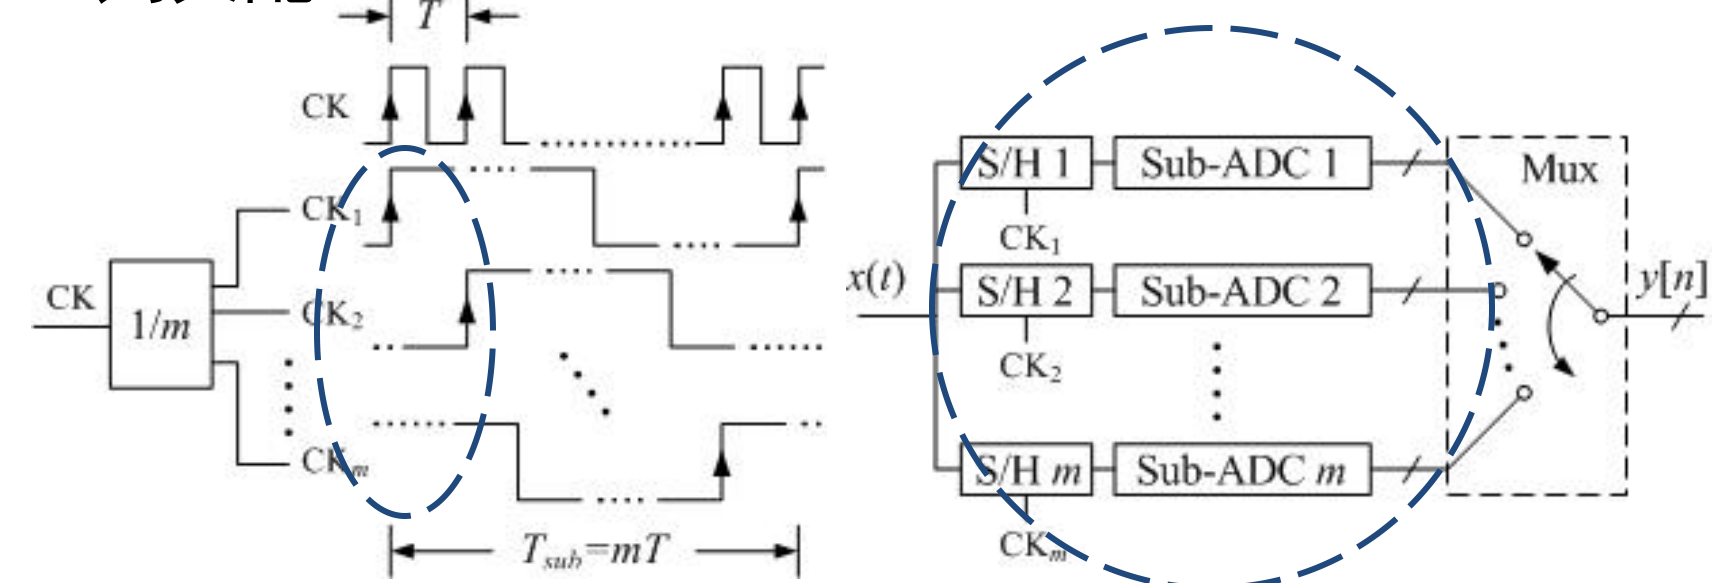
\includegraphics[width=1\textwidth]{figure/circuit3.png}
			\caption{时间交织原理及时序图} \label{fig:circuit3}
		\end{figure}
		\noindent
		\textbf{\textit{同样,注意建模设计要点:不同的通道间误差及其各自与频谱的对应关系}}
		在此,我们会首先回顾课上以两通道为例的失配,再将其推广到多通道,并研究不同通道间误差与频谱各自的对应关系。

		\subsubsection{失调失配}
		\textbf{以2通道为例,输入为 $x(t) = \cos(\omega t + \phi)$}
		\begin{itemize}
			\item \textbf{失调失配}:$x(t) = \cos(\omega t + \phi) + OS$
			\begin{itemize}
				\item 存在\textcolor{red}{失调}失配,$\Delta OS = OS_A - OS_B \neq 0$
				\item 量化结果:
				\[
				y[n] = \cos(\omega nT + \phi) + OS + \frac{\Delta OS}{2} \cos\left(\frac{\omega_s}{2} nT \right)
				\]
			\end{itemize}
		\end{itemize}
		\underline{\textbf{接下来,推广到多通道失调失配:}}
		\begin{equation}
			\begin{gathered}
				x_s(t)=x(t)+O(t)\\
				 \quad f_{I L}=k f_s / M \quad \text { where } k=0,1,2,3 \ldots, M-1 \\
				P_N=\frac{1}{M} \sum_{i=0}^{M-1}\left|O_i\right|^2
			\end{gathered}
		\end{equation}
		
		
		
		\subsubsection{增益失配}
		\textbf{增益失配}:$x(t) = G \cdot \cos(\omega t + \phi)$
		\begin{itemize}
			\item 存在\textcolor{red}{增益}失配,$\Delta G = G_A - G_B \neq 0$
			\item 量化结果:
			\[
			y[n] = G \cos(\omega nT + \phi) + \frac{\Delta G}{2} \cos\left[ \left(\omega - \frac{\omega_s}{2} \right) nT + \phi \right]
			\]
		\end{itemize}
		\underline{\textbf{接下来,推广到多通道增益失配:}}
		\begin{equation}
			\begin{gathered}
				x_s(t)=x(t) \times G(t) \\
				 f_{\text {Gain }} =k f_s / M \\
				f_{\text {IL }}=f_{\text {Gain }} \pm f_{\text {in }}= \pm f_{\text {in }}+\frac{k}{M} f_s \\
				 P_{\text {Total }}  =\frac{1}{2 M} \sum_{i=0}^{M-1}\left|G_i\right|^2
			\end{gathered}
		\end{equation}
		
		\subsubsection{时钟偏差}
		\textbf{采样时刻偏差}:$x(t) = \cos(\omega t + \phi + \Delta T)$
		\begin{itemize}
			\item 存在\textcolor{red}{采样时刻偏差},$\Delta T$
			\item 量化结果:
			\[
			y[n] = \cos\left(\frac{\omega \Delta T}{2}\right) \cos(\omega nT + \phi) + \sin\left(\frac{\omega \Delta T}{2}\right) \sin\left[\left(\omega - \frac{\omega_s}{2} \right) nT + \phi \right]
			\]
		\end{itemize}
		\underline{\textbf{接下来,推广到多通道采样时刻偏差:}}
		\begin{equation}
			\begin{array}{lr}
				x_s(t)=x(t-\delta t) & x_s(t)=\sin \left(2 \pi f_{i n} t\right) \cos \left(2 \pi f_{i n} \delta t\right)-\cos \left(2 \pi f_{i n} t\right) \sin \left(2 \pi f_{i n} \delta t\right) \\
				x(t)=\sin \left(2 \pi f_{i n} t\right) & x_s(t) \cong \sin \left(2 \pi f_{i n} t\right)-\left(2 \pi f_{i n} \delta t\right) \cos \left(2 \pi f_{i n} t\right) \\
				x_s(t)=\sin \left(2 \pi f_{i n} t-2 \pi f_{i n} \delta t \right) & f_{I L}= \pm f_{i n}+f_{\delta t}= \pm f_{i n}+\frac{k}{M} f_s \nonumber
			\end{array}
		\end{equation}
		
		\begin{equation}
			P_N=\frac{\left(2 \pi f_{i n}\right)^2}{2 M} \sum_{i=0}^{M-1}\left|\delta t_i\right|^2
		\end{equation}
		
		
		\subsubsection{带宽失配(但这个在本模型中未体现)}
		\textbf{带宽失配}:$x(t) = H(\omega) \cdot \cos(\omega t + \phi)$
		\begin{itemize}
			\item 存在\textcolor{red}{带宽}失配,$\Delta H(\omega) = H_A(\omega) - H_B(\omega) \neq 0$
			\item 量化结果:
			\[
			y[n] = H(\omega) \cos(\omega nT + \phi) + \frac{\Delta H(\omega)}{2} \cos\left[\left( \omega - \frac{\omega_s}{2} \right) nT + \phi \right]
			\]
		\end{itemize}
		\underline{\textbf{带宽失配未在本模型中加以考虑,只是在此做一个简单的说明}}
		
		\subsection{时间交织失配误差总结}
		\begin{flushleft}
			\begin{table}[H]
					\caption{时间交织失配误差总结}
					\begin{tabular}{|l|l|l|}
					\hline \textbf{Type of mismatch} & \textbf{Effect on input} & \textbf{Spur location} \\
					\hline Offset mismatch & Additive effect & $f_{\text {IL }}=\frac{k}{M} f_s$ \\
					\hline Gain mismatch & Amplitude modulation & $f_{\text {IL }}= \pm f_{\text {in }}+\frac{k}{M} f_s$ \\
					\hline Timing mismatch & Phase modulation & $f_{\text {IL }}= \pm f_{\text {in }}+\frac{k}{M} f_s$ \\
					\hline Bandwidth mismatch & Freq.-dependent amplitude and phase modulation & $f_{I L}= \pm f_{\text {in }}+\frac{k}{M} f_s$ \\
					\hline
				\end{tabular}
			\end{table}
		\end{flushleft}
		
		\subsection{关于电荷重分配}
			如图\ref{fig:cap}所示,采用电荷重分配结构。图中得到的参考电压可以表示为
			\begin{equation}
				V_{\text {out }}=\frac{\sum_{i=0}^{B-1} b_i 2^i C}{2^B C+C_P} V_{\text {ref }}
			\end{equation}
			
			\begin{figure}[H]
				\centering
				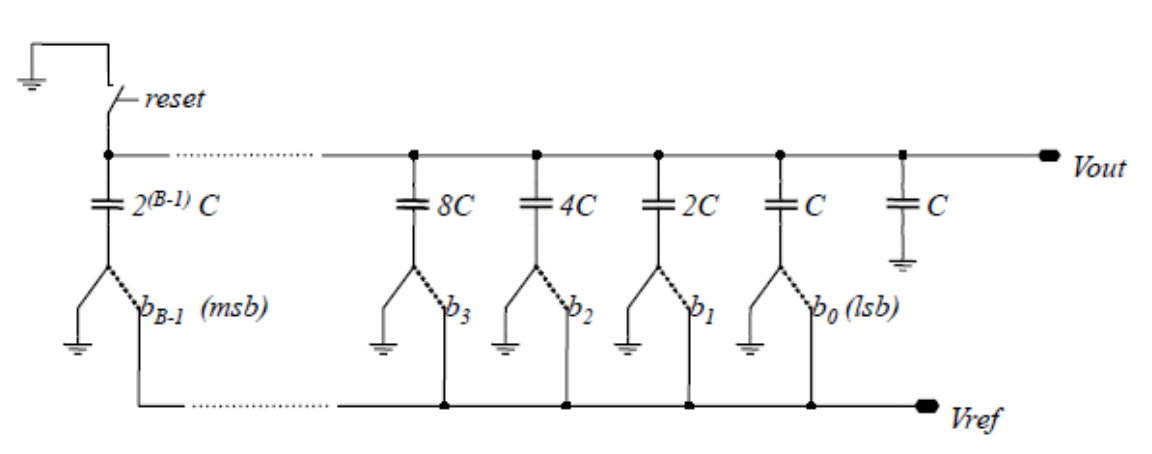
\includegraphics[width=1\textwidth]{figure/cap.png}
				\caption{电荷重分配基本结构} \label{fig:cap}
			\end{figure}
			
			\subsubsection{基本原理}
			\begin{itemize}
				\item 电荷重分配是逐次逼近型 ADC 中常用的 DAC 实现方式。
				\item 利用一组按二进制权重排列的电容阵列,通过切换其下极板的连接(Vref/GND)来实现数字码控制下的输出电压。
				\item 工作过程基于电荷守恒定律,上极板节点浮空,依赖电荷转移来建立目标电压。
			\end{itemize}
			
			\subsubsection{工作阶段}
			\begin{enumerate}
				\item \textbf{采样阶段(Sampling)}:
				\begin{itemize}
					\item 所有电容上下极板接地,或使用顶极板采样(Flip-around结构)。
					\item 输入信号通过开关加载到电容阵列上。
				\end{itemize}
				\item \textbf{保持阶段(Hold)}:
				\begin{itemize}
					\item 上极板节点浮空,下极板根据比较结果逐位切换。
					\item 每一次切换后输出电压会逼近目标值的一半。
				\end{itemize}
			\end{enumerate}
			
			\subsubsection{设计注意事项}
			\begin{itemize}
				\item 上极板寄生电容 $C_p$ 影响输出精度,若与输出电压有关会造成非线性。
				\item 使用桥接电容可减小电容总数(但本次课程设计中未采用)。
				\item 可引入冗余设计以修正高位误差。
			\end{itemize}
		
		\subsection{关于差分结构}
		注意:本课程设计采用差分结构,如图\ref{fig:diff}所示。
			\begin{figure}[H]
				\centering
				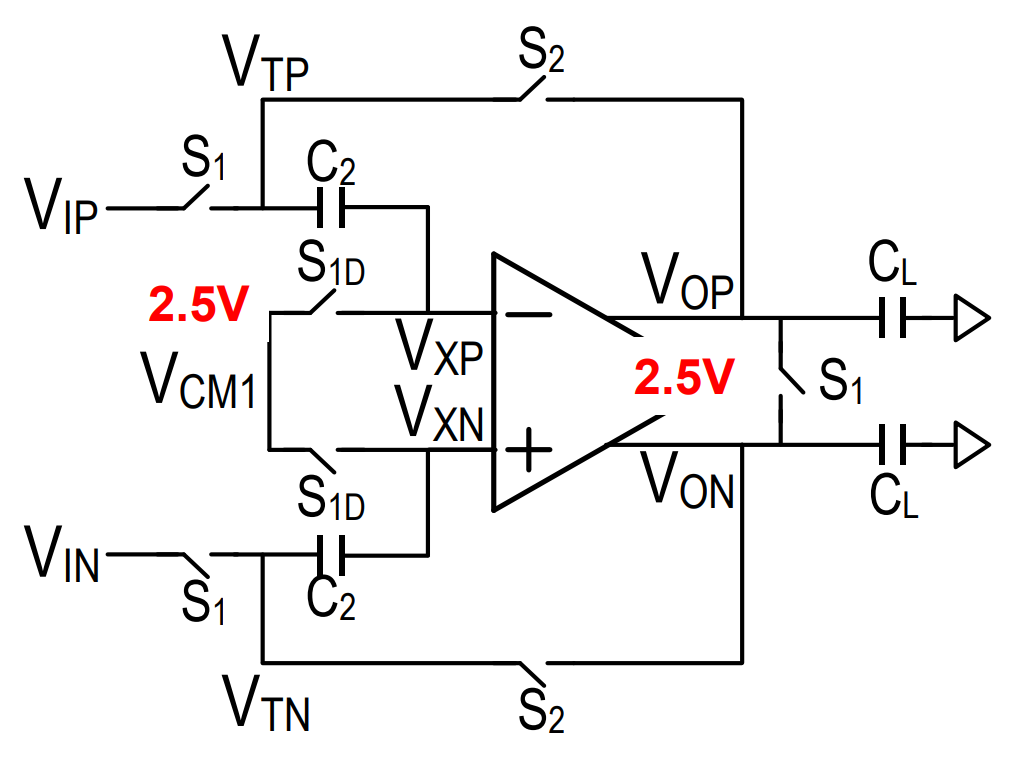
\includegraphics[width=0.6\textwidth]{figure/diff.png}
				\caption{差分结构flip-around图} \label{fig:diff}
			\end{figure}
		
		
			\subsubsection{结构特点}
			\begin{itemize}
				\item 利用一对对称电路分别处理正负输入信号,输出差分信号。
				\item 能有效抑制共模干扰、offset 电压、时钟跳变电荷注入等问题。
			\end{itemize}
			
			\subsubsection{在 Flip-Around T/H 中的应用}
			\begin{itemize}
				\item 差分结构配合电荷翻转采样(Flip-Around)结构,能抵消底极板开关注入误差。
				\item 差分结构中反馈因子为 1,增益为 1,简化了运放需求。
				\item 若采用开环复位,需注意信号共模在跟踪与保持相位的一致性。
			\end{itemize}
			
			\subsubsection{非理想性考虑}
			\begin{itemize}
				\item \textbf{开环增益}:有限增益造成误差 $V_{OUT} = \frac{V_{IN}}{1 + A^{-1}}$。
				\item \textbf{失调电压 $V_{OS}$}:导致输出恒定偏移 $V_{OUT} = V_{IN} + V_{OS}$。
				\item \textbf{寄生电容 $C_P$}:若恒定,可视为增益误差;若非恒定则引入非线性。
			\end{itemize}
			
			\subsubsection{扩展应用}
			\begin{itemize}
				\item \textbf{T/H + 放大}:通过电荷重分配结构实现电压增益,增益由电容比 $C_1/C_2$ 决定。
				\item \textbf{T/H + 求差或求和}:通过多个电容节点在跟踪和保持相位切换实现差分计算。
				\item 差分结构能推广至所有上述电路,并可通过精密电容匹配提高精度。
			\end{itemize}
			
\newpage		
\section{MATLAB建模和仿真}
	\subsection{模型介绍}
	整体模型仿照硬件的结构进行搭建,主要包括以下几个部分:
	\begin{itemize}
		\item 顶层模型:
		实现整个时钟交织流水线SAR ADC的功能仿真。定义了ADC的整体参数和可能的噪声和失配,并生成测试用的正弦信号。
		ADC整体采用差分结构,因此需要生成两个共模相同,差模相反的正弦信号。
		模型首先对信号进行时钟交织的采样,采样时考虑了多通道间的时钟失配、增益失配、偏移量和kT/C噪声,将这些非理想因素叠加到输入信号中;
		接着调用多个流水线SAR ADC对多路采样数据进行并行化处理,考虑到了流水线ADC的各种噪声和失配,具体的因素会在每个模块中介绍;
		最后使用多路选择器将各个通道的量化结果整合得到更高采样率的量化结果。
		
		\item 流水线SAR ADC模型函数:
		实现流水线SAR ADC的功能仿真,以函数的形式被顶层模型调用。采用了两级流水的结构,并设置1位冗余位。
		考虑到噪声和失真的影响,采用了7位/9位的分布,使得最终的ENOB可以达到12位的设计要求。

		模型内部首先根据两级SAR ADC的位数求出两级所需要的电容值,并生成相应的电容阵列,电容阵列考虑到了寄生电容和电容大小失配。
		需要注意的是,第一级的余差在比较完成后还需要进一步缩小余差传递到第二级,
		而第二级的最后的余差在比较完成后不需要进一步处理,因此两级SAR ADC的实现方式有所不同,需要的电容数量也有所不同。
		具体而言,如果两级SAR ADC分别为N1位和N2位,则第一级SAR ADC的电容阵列需要N1+1个电容,而第二级SAR ADC的电容阵列只需要N2个电容。
		
		两级SAR ADC之间由一个余差放大器连接,使用反馈的形式控制余差的放大,将放大后的结果作为第二级SAR ADC的输入。

		最终的结果由两级SAR ADC的输出拼接得到。计算时将两级的冗余位重叠相加,并减去固定的偏移量得到最终的量化结果,输出到顶层模块进行多路整合。

		\item SAR ADC模型函数:
		模型的工作过程仿照SAR ADC的工作原理,使用循环模拟逐次逼近的过程,每次循环对输入的差分信号进行比较,并进行相应调整,考虑了比较器的失调和噪声。
		两级SAR ADC由于之前提到的原因,存在一些差别,需要分别设计。
		第一级ADC的电容阵列需要N1+1个电容,第二级ADC的电容阵列只需要N2个电容,并且第一级对输出余差电压的调整次数也比第二级多一次。其余部分两级完全相同。

		\item ResAmp模型函数:
		余差放大器将两个输入信号按照闭环增益进行放大,根据放大器的增益带宽积进行滤波后输出到第二级SAR ADC进行处理。
		输入的信号叠加了放大器的噪声和失调,闭环增益的计算也包含了有限增益带来的非线性因素。

		\item 静态参数测试函数
		实现对ADC静态参数的测试,包括DNL、INL指标的计算。由于输入是正弦信号,理想的histogram并不是均匀分布,而是呈“浴盆状”的分布曲线。
		函数通过使用大量数据模拟得到理想的概率分布,再用实际得到的概率分布与理想分布相减得到DNL,对DNL积分得到INL。

		\item 动态参数测试函数
		实现对ADC动态参数的测试,包括SNR、SFDR、THD、SNDR和ENOB指标的计算。函数通过对输入的正弦信号进行FFT变换,得到频谱图,
		去除DC分量后找到能量最大的频率作为主频,将主频乘以整数倍的频率作为谐波,取2-5次谐波进行计算。
		计算主频和谐波的功率比得到THD,将2次谐波功率与主频功率的比得到SFDR。
		去除DC、主频和谐波后,计算剩余部分的功率就是噪声功率,主频功率与噪声功率之比就是SNR。
		主频功率比上噪声功率与谐波功率之和就是SNDR,由此可以计算出ENOB。由于各种噪声和失真,ENOB小于最初设计的15位,但仍然满足12位的要求。

	\end{itemize}
	\subsection{仿真参数}
	在本节中,我们将对上述模型进行仿真,主要关注以下几个方面的参数设置:
	\subsubsection{模型参数}
	\begin{itemize}
		\item \textbf{采样频率}:$f_s = 2 \text{GHz}$
		\item \textbf{参考电压幅度}:$V_{ref} = 1.8V$
		\item \textbf{共模电压}:$V_{cm} = 0.9V$
		\item \textbf{ADC位数}:$N = 13$,这是ADC的理想位数。
		\item \textbf{通道数}:$M = 4$,这是时间交织ADC的通道数。
		\item \textbf{非理想指标}:包括时钟jitter、增益失配、偏移失调等,这些参数将在仿真中逐步调整。
	\end{itemize}

	\subsubsection{采样与输入信号参数}
	\begin{itemize}
		\item \textbf{采样点数}:$num = 2^{22}$,这是整个ADC的采样点数。由于理想位数为15位,为了完整测量,采样了$2^{22}$。
		\item \textbf{输入信号频率}:$f_{in} = \frac{1431}{num} * fs$,未超过奈奎斯特频率,且与采样频率$f_s$互质,以免DNL测量出现-1。同时采样$num$点正好是整周期,可以不进行加窗。
		\item \textbf{输入信号幅度}:$V_{in} = 1.0$,这是输入正弦信号的幅度。
	\end{itemize}

	由于许多非线性使用randn()函数生成,因此每次仿真结果会有所不同。下仅为展示,实际仿真结果会有一定的随机性。同时由于非理想的取值不一定非常合理,因此不同非理想因素之间相互比较不一定能作为准确结果

	\subsection{仿真结果}
	在本节中,我们将展示基于上述模型和参数在不同情况下的仿真结果,包括静态参数和动态参数的测试结果。
	\subsubsection{理想情况}
	在没有任何失配、失调等情况下,我们可以得到理想的ADC性能。可以看到最差DNL为0.0303LSB,最差INL为0.0167LSB,SNR为92.06dB,SNDR为92.06dB,SFDR为124.22dB,THD为158.68dB,ENOB为15bit。

	可见理想情况的ADC的ENOB是正确的,由于级间放大器开环增益无法设置为正无穷,因此一定存在THD,但影响不大。DNL与INL曲线十分合理,没有出现失码情况,但是由于采样点仍不够多,精度并不高。
		\begin{figure}[H]
			\centering
			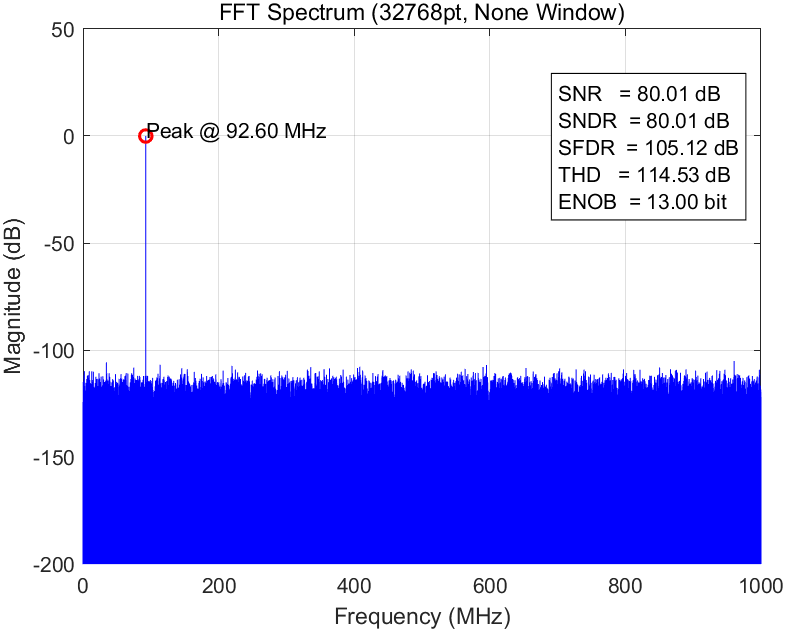
\includegraphics[width=0.7\textwidth]{pic/ideal/DFT.png}
			\caption{理想情况下的动态特性} 
		\end{figure}

		\begin{figure}[H]
			\centering
			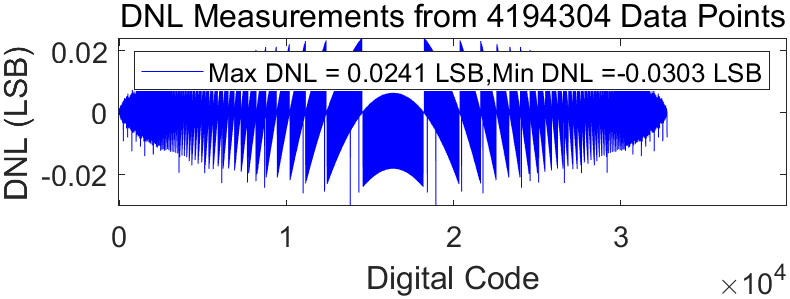
\includegraphics[width=0.7\textwidth]{pic/ideal/DNL.png}
			\caption{理想情况下的DNL} 
		\end{figure}

		\begin{figure}[H]
			\centering
			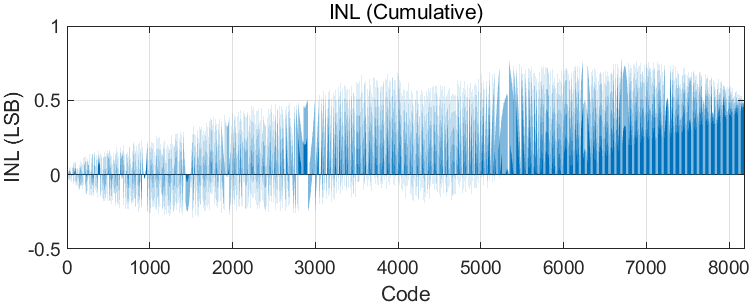
\includegraphics[width=0.7\textwidth]{pic/ideal/INL.png}
			\caption{理想情况下的INL} 
		\end{figure}

		\begin{figure}[H]
			\centering
			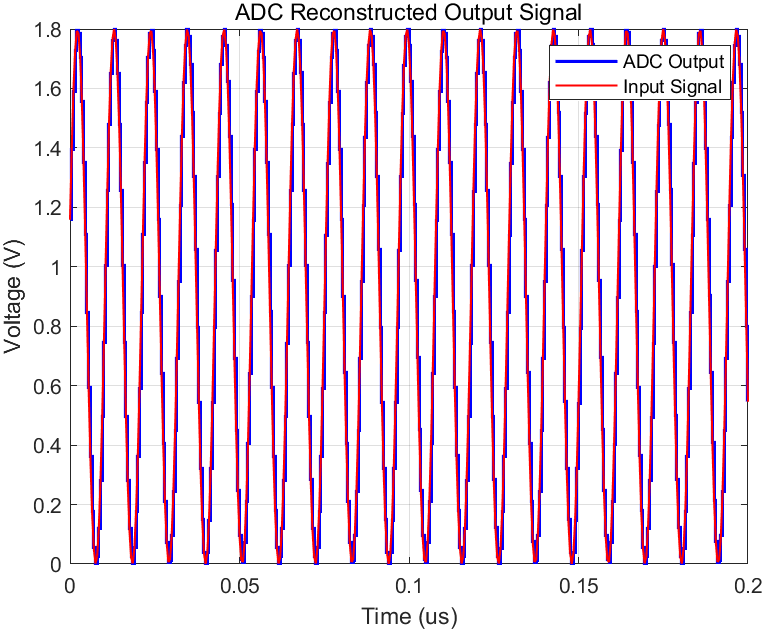
\includegraphics[width=0.7\textwidth]{pic/ideal/inout.png}
			\caption{理想情况下的输入输出对比} 
		\end{figure}

	\subsubsection{TI mismatch}
	\begin{itemize}
		\item \textbf{失调失配} 设置四个通道各自有$Mis_{OS} = 0.5 * LSB * randn()$;此时ADC性能。可以看到最差DNL为0.814LSB,最差INL为0.814LSB,SNR为91.15dB,SNDR为91.15dB,SFDR为98.33dB,THD为146.65dB,ENOB为14.85bit。

		可以从DFT图中看到明显的谐波失真。四通道的失真出现频率难以推导。DNL整体较为平稳,只有最后变为-0.814LSB。
		\begin{figure}[H]
			\centering
			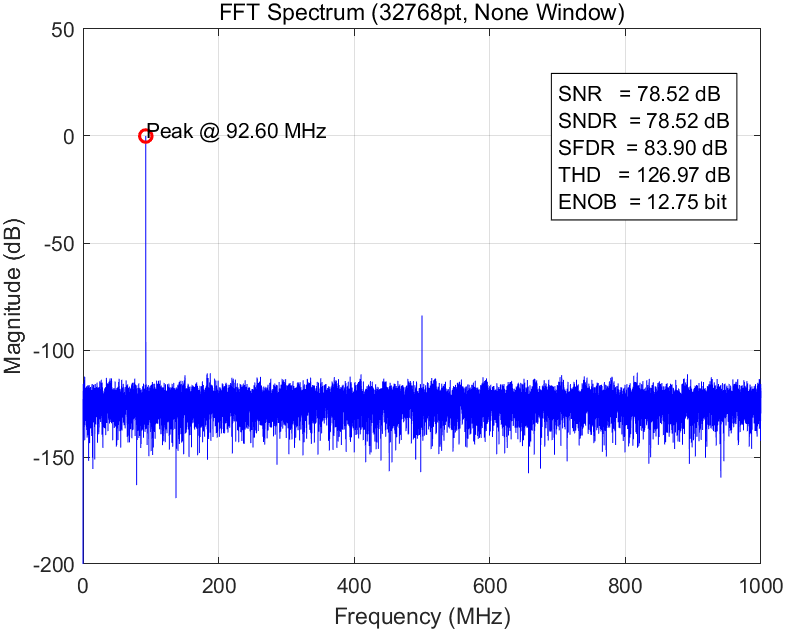
\includegraphics[width=0.7\textwidth]{pic/TIOS/DFT.png}
			\caption{通道内存在失调失配下的动态特性} 
		\end{figure}

		\begin{figure}[H]
			\centering
			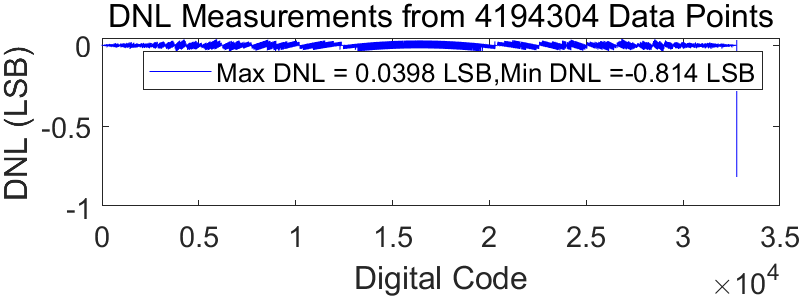
\includegraphics[width=0.7\textwidth]{pic/TIOS/DNL.png}
			\caption{通道内存在失调失配下的DNL} 
		\end{figure}

		\begin{figure}[H]
			\centering
			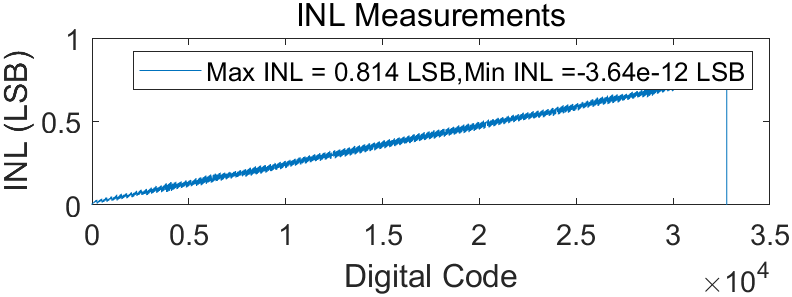
\includegraphics[width=0.7\textwidth]{pic/TIOS/INL.png}
			\caption{通道内存在失调失配下的INL} 
		\end{figure}

		\item \textbf{增益失配} 设置四个通道各自有$Mis_{Gain} = 1 + 0.2 * randn()$;此时ADC性能。可以看到最差DNL为0.989LSB,最差INL为1.07LSB,SNR为91.4dB,SNDR为91.4dB,SFDR为101.82dB,THD为145.5dB,ENOB为14.89bit。
		
		可以从DFT图中看到明显的谐波失真。四通道的失真出现频率难以推导。DNL整体较为平稳,只有最后变为-0.989LSB,接近失码。
		\begin{figure}[H]
			\centering
			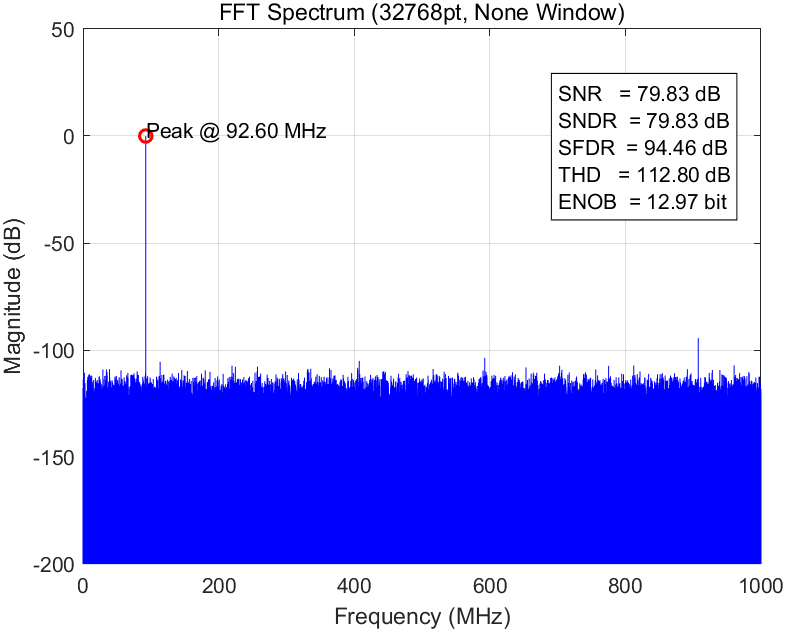
\includegraphics[width=0.7\textwidth]{pic/TIG/DFT.png}
			\caption{通道内存在增益失配下的动态特性} 
		\end{figure}

		\begin{figure}[H]
			\centering
			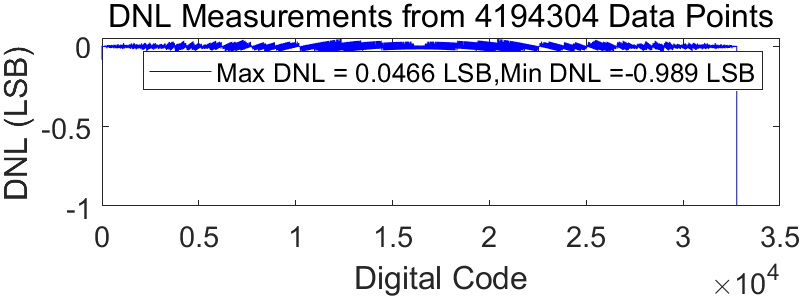
\includegraphics[width=0.7\textwidth]{pic/TIG/DNL.png}
			\caption{通道内存在增益失配下的DNL} 
		\end{figure}

		\begin{figure}[H]
			\centering
			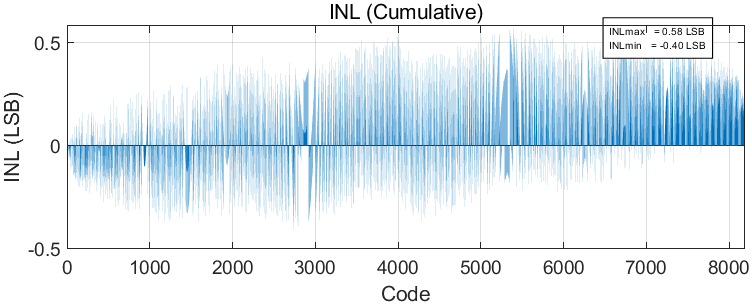
\includegraphics[width=0.7\textwidth]{pic/TIG/INL.png}
			\caption{通道内存在增益失配下的INL} 
		\end{figure}

		\item \textbf{时钟偏差} 设置四个通道各自有$Mis_{Clk} = 0.05 * 1/fs * randn()$;可以看到最差DNL为0.0222LSB,最差INL为0.0235LSB,SNR为79.98dB,SNDR为79.98dB,SFDR为84.98dB,THD为149.21dB,ENOB为12.99bit。
		
		时钟偏差带来的负面影响主要体现在SNR和SNDR上,DNL和INL的影响较小。可以从DFT图中看到明显的谐波失真。四通道的失真出现频率难以推导。DNL整体较为平稳,只有最后变为-0.0222LSB。
		\begin{figure}[H]
			\centering
			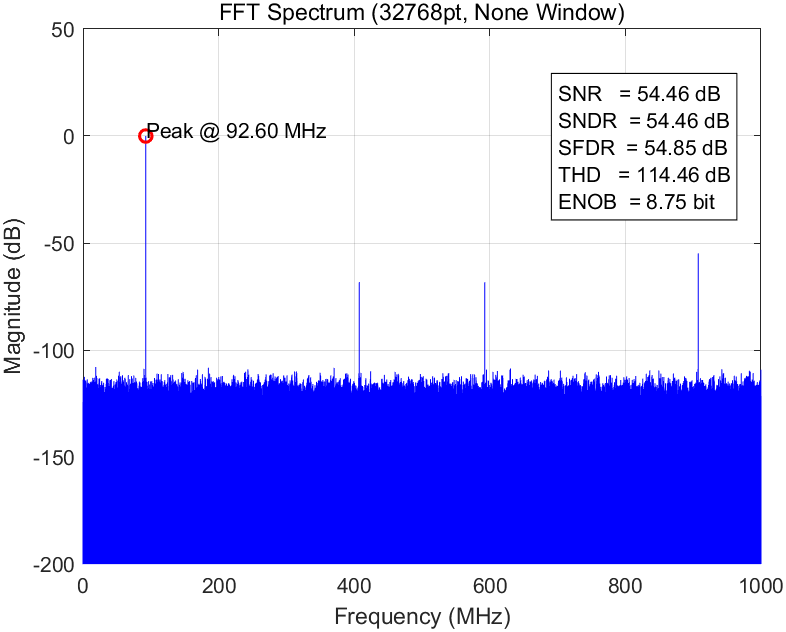
\includegraphics[width=0.7\textwidth]{pic/TIC/DFT.png}
			\caption{通道间存在时钟偏差下的动态特性} 
		\end{figure}

		\begin{figure}[H]
			\centering
			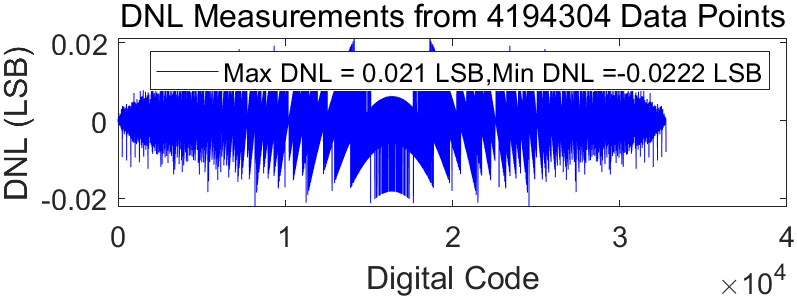
\includegraphics[width=0.7\textwidth]{pic/TIC/DNL.png}
			\caption{通道间存在时钟偏差下的DNL} 
		\end{figure}

		\begin{figure}[H]
			\centering
			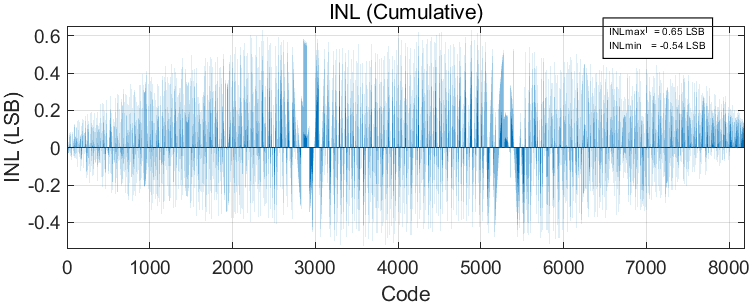
\includegraphics[width=0.7\textwidth]{pic/TIC/INL.png}
			\caption{通道间存在时钟偏差下的INL} 
		\end{figure}
	\end{itemize}

	\subsubsection{pipelined-SAR ADC级间运放误差}
	\begin{itemize}
		\item \textbf{有限增益误差(级间增益误差)} 级间增益误差可以通过改变级间增益放大器的开环增益来实现,当开环增益非正无穷时,级间增益为理想的$2^6=64$。将开环增益改为80dB,实际级间增益为$\frac{10000}{1+10000*\frac{1}{2^6}}=63.59$。
		
		可以看到最差DNL为0.832LSB,最差INL为1.62LSB,SNR为86.35dB,SNDR为86.35dB,SFDR为104.63dB,THD为159.92dB,ENOB为14.05bit。
		
		可以从DFT图中看出,并没有什么谐波失真,但是DNL和INL图像不再理想,DNL出现了等间隔的最低点(单方向性),这是由于每隔低位就会出现大的失调,符合逻辑。
		\begin{figure}[H]
			\centering
			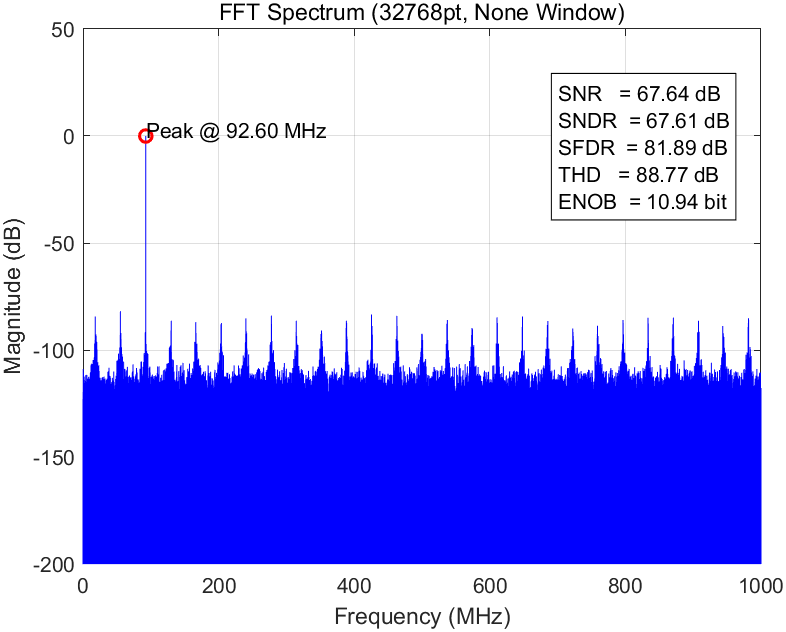
\includegraphics[width=0.7\textwidth]{pic/Av/DFT.png}
			\caption{有限增益误差下的动态特性} 
		\end{figure}

		\begin{figure}[H]
			\centering
			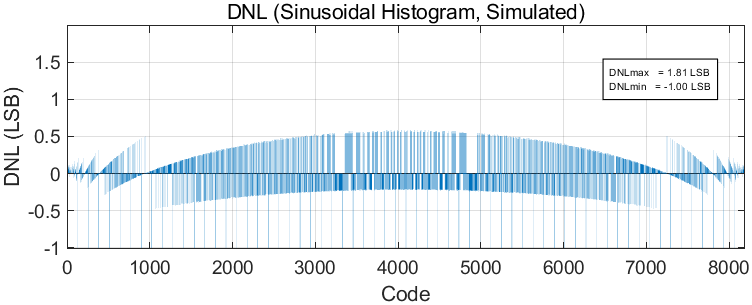
\includegraphics[width=0.7\textwidth]{pic/Av/DNL.png}
			\caption{有限增益误差下的DNL} 
		\end{figure}

		\begin{figure}[H]
			\centering
			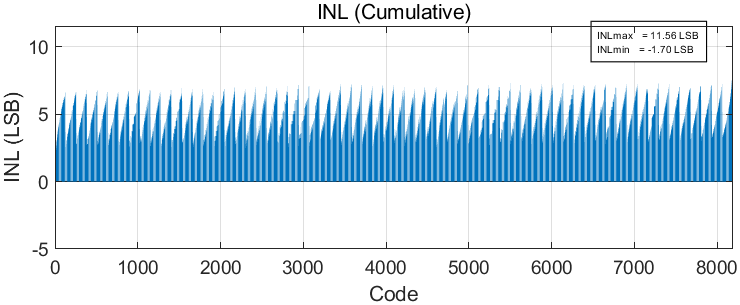
\includegraphics[width=0.7\textwidth]{pic/Av/INL.png}
			\caption{有限增益误差下的INL} 
		\end{figure}

		\item \textbf{有限带宽误差} 理想情况时级间增益放大器的带宽为$10GHz$,现将带宽设置为为$0.1GHz$。
		
		可以看到最差DNL为0.419LSB,最差INL为0.264LSB,SNR为90.15dB,SNDR为90.15dB,SFDR为108.80dB,THD为160.71dB,ENOB为14.68bit。
		
		可以从DFT图中看出,并没有什么谐波失真,但是DNL和INL图像不再理想,DNL等间隔出现最高点与最低点,不再是单一的,符合逻辑。
		\begin{figure}[H]
			\centering
			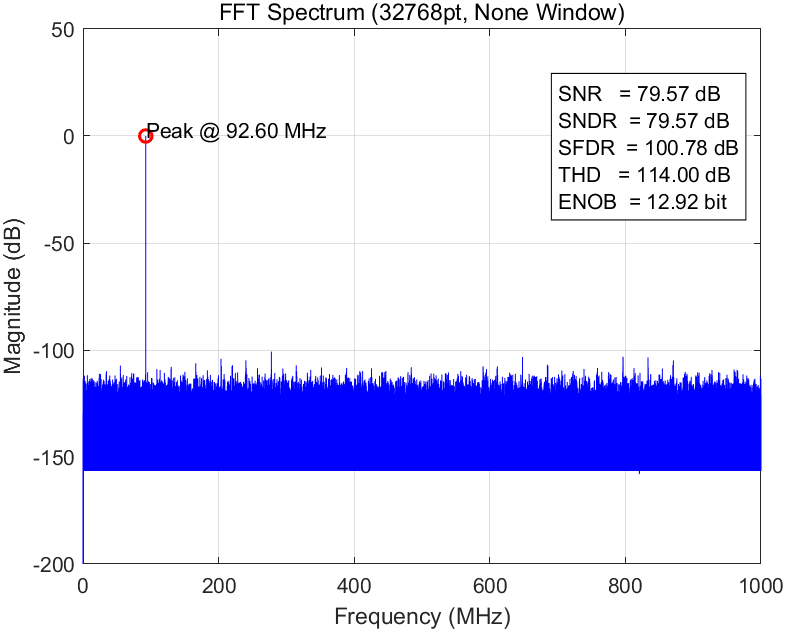
\includegraphics[width=0.7\textwidth]{pic/GBW/DFT.png}
			\caption{有限带宽误差下的动态特性} 
		\end{figure}

		\begin{figure}[H]
			\centering
			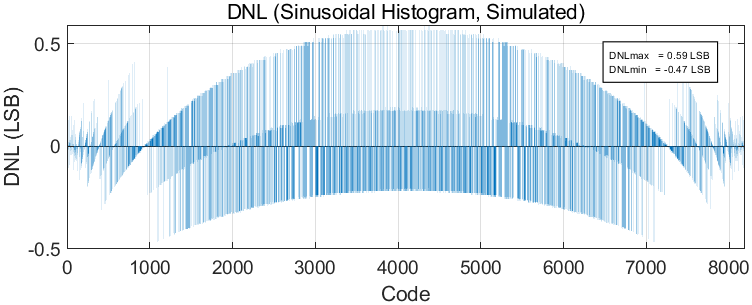
\includegraphics[width=0.7\textwidth]{pic/GBW/DNL.png}
			\caption{有限带宽误差下的DNL} 
		\end{figure}

		\begin{figure}[H]
			\centering
			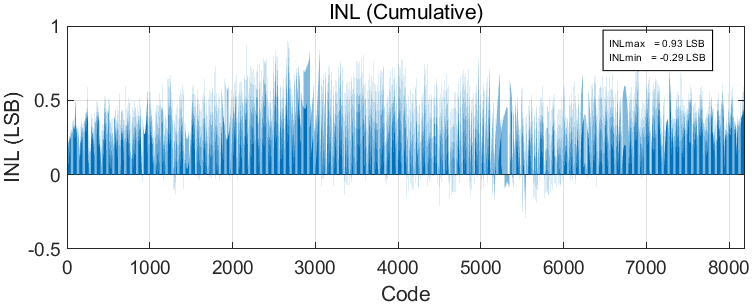
\includegraphics[width=0.7\textwidth]{pic/GBW/INL.png}
			\caption{有限带宽误差下的INL} 
		\end{figure}

		\item \textbf{运放失调} 将失调调为0.001V。
		
		可以看到最差DNL为0.866LSB,最差INL为0.866LSB,SNR为92.06dB,SNDR为92.06dB,SFDR为126.68dB,THD为161.51dB,ENOB为15bit。
		
		可以清楚的看到ENOB并没有任何的下降,这是合理的,因为有冗余位的存在,较小的offset并不会产生影响。DNL除了最后,基本也符合理想情况,每个码所占略微有些变化。

		\begin{figure}[H]
			\centering
			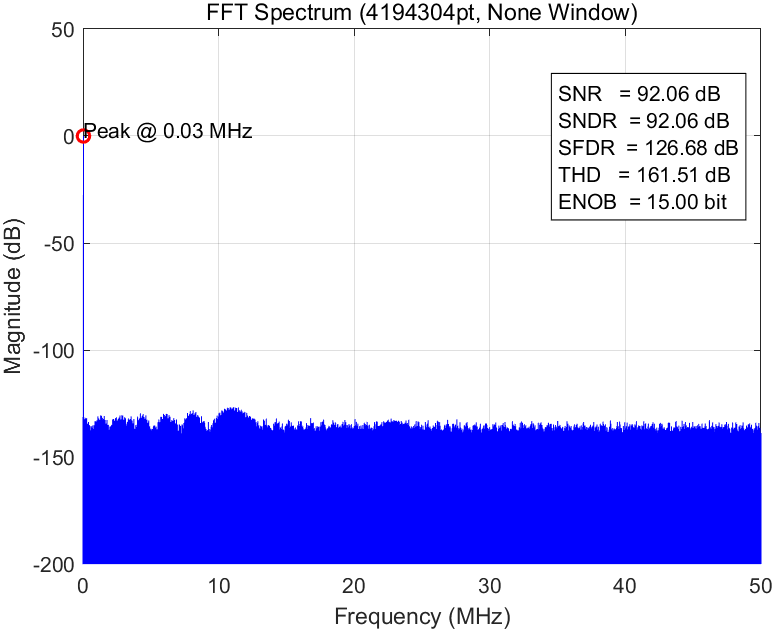
\includegraphics[width=0.7\textwidth]{pic/Avno/DFT.png}
			\caption{存在运放失调时的动态特性} 
		\end{figure}

		\begin{figure}[H]
			\centering
			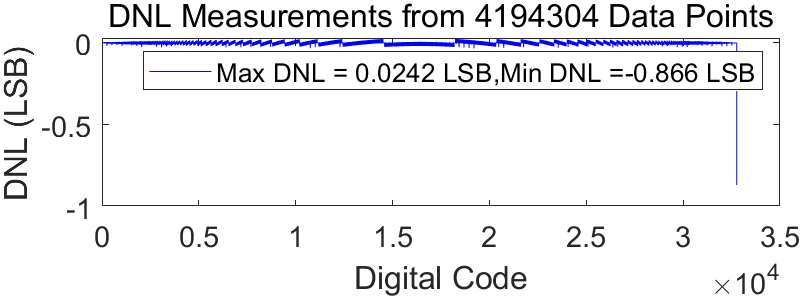
\includegraphics[width=0.7\textwidth]{pic/Avno/DNL.png}
			\caption{存在运放失调时的DNL} 
		\end{figure}

		\begin{figure}[H]
			\centering
			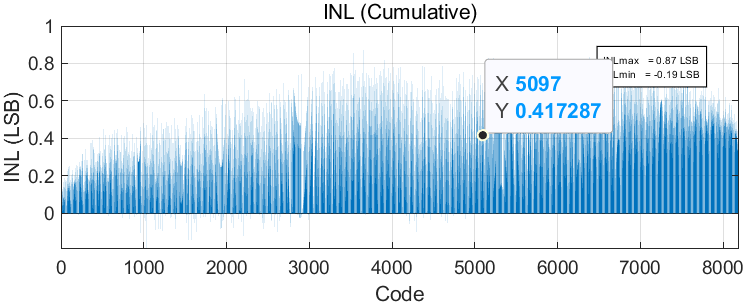
\includegraphics[width=0.7\textwidth]{pic/Avno/INL.png}
			\caption{存在运放失调时的INL} 
		\end{figure}

	\end{itemize}

\subsubsection{SAR ADC非理想}
	\begin{itemize}
		\item \textbf{比较器失调} 将失调调为0.005V。
		可以看到最差DNL为0.719LSB,最差INL为0.719LSB,SNR为92.07dB,SNDR为92.07dB,SFDR为124.89dB,THD为160.76dB,ENOB为15bit。
		
		可以清楚的看到ENOB并没有任何的下降,这是合理的,因为有冗余位的存在,较小的offset并不会产生影响。DNL除了最后,基本也符合理想情况,每个码所占略微有些变化。
		\begin{figure}[H]
			\centering
			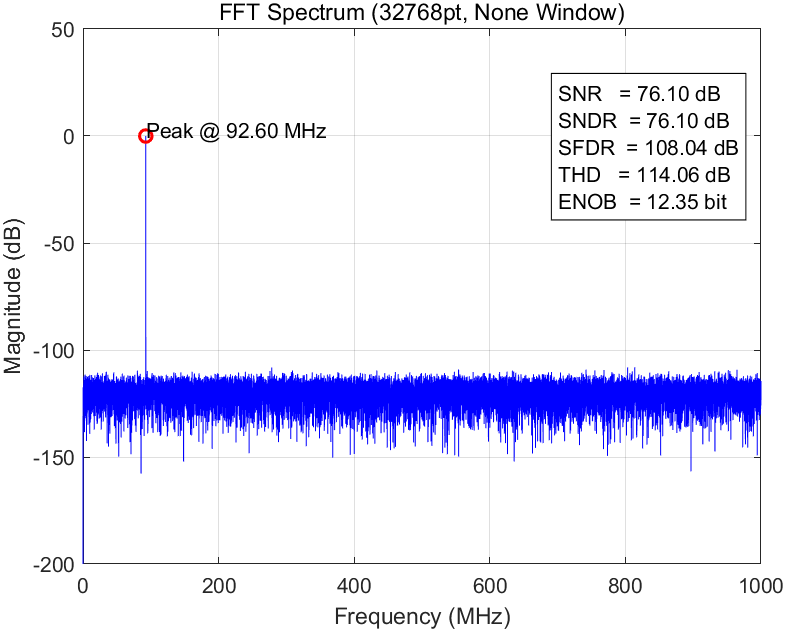
\includegraphics[width=0.7\textwidth]{pic/Comno/DFT.png}
			\caption{存在比较器失调的动态特性} 
		\end{figure}

		\begin{figure}[H]
			\centering
			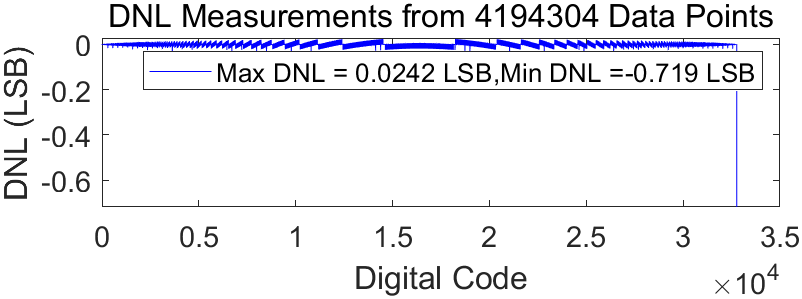
\includegraphics[width=0.7\textwidth]{pic/Comno/DNL.png}
			\caption{存在比较器失调的DNL} 
		\end{figure}

		\begin{figure}[H]
			\centering
			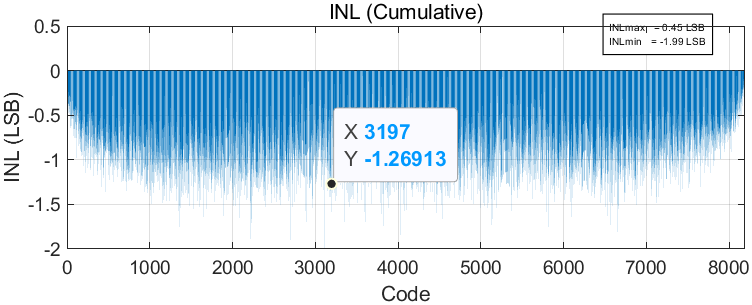
\includegraphics[width=0.7\textwidth]{pic/Comno/INL.png}
			\caption{存在比较器失调的INL} 
		\end{figure}

		\item \textbf{寄生电容} 先将第一级的寄生电容调为$Cp_{p1}  = 5fF $、$ Cp_{n1} = 5fF;$ 
		
		可以看到最差DNL为0.0284LSB,最差INL为0.0259LSB,SNR为92.07dB,SNDR为92.07dB,SFDR为124.48dB,THD为154.85dB,ENOB为15bit。
		
		可以清楚的看到ENOB并没有任何的下降,这是合理的,由于存在冗余,寄生电容又只会产生固定的偏差,可以依靠冗余将固定偏差消除。DNL与INL也基本与理想无异。
		\begin{figure}[H]
			\centering
			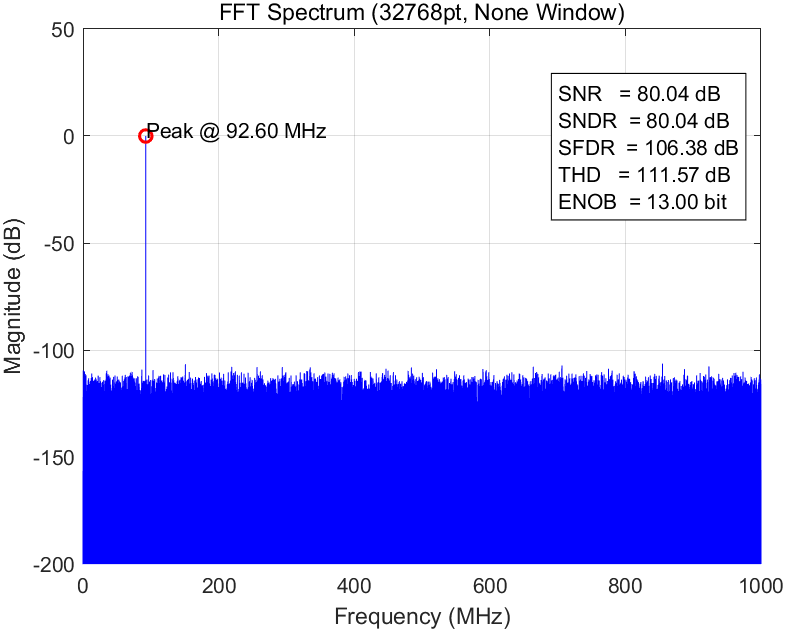
\includegraphics[width=0.7\textwidth]{pic/Co/DFT1.png}
			\caption{第一级寄生电容的动态特性} 
		\end{figure}

		\begin{figure}[H]
			\centering
			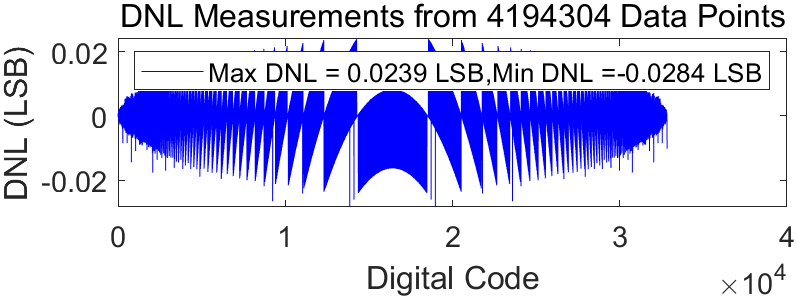
\includegraphics[width=0.7\textwidth]{pic/Co/DNL1.png}
			\caption{第一级寄生电容的DNL} 
		\end{figure}

		\begin{figure}[H]
			\centering
			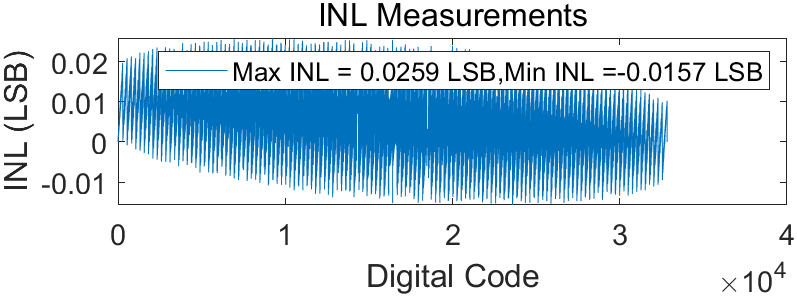
\includegraphics[width=0.7\textwidth]{pic/Co/INL1.png}
			\caption{第一级寄生电容的INL} 
		\end{figure}

		再将第二级的寄生电容调为$Cp_{p2}  = 5fF $、$ Cp_{n2} = 5fF;$
		
		可以看到最差DNL为0.994LSB,最差INL为5.34LSB,SNR为77.81dB,SNDR为77.81dB,SFDR为94.75dB,THD为157.67dB,ENOB为12.63bit。
		
		在第二级,后面并没有冗余,寄生电容的误差出现,非线性与线性度都出现了大幅下降。DNL与INL出现了严重的恶化,SNR与SNDR大幅下降。
		\begin{figure}[H]
			\centering
			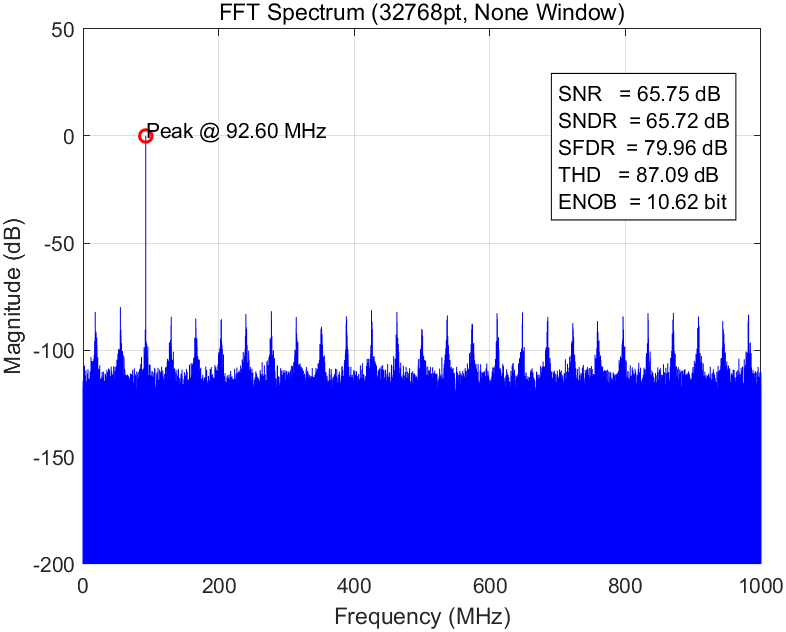
\includegraphics[width=0.7\textwidth]{pic/Co/DFT2.png}
			\caption{第二级寄生电容的动态特性}
		\end{figure}

		\begin{figure}[H]
			\centering
			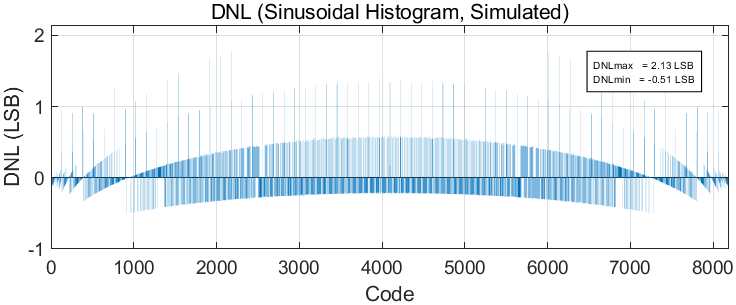
\includegraphics[width=0.7\textwidth]{pic/Co/DNL2.png}
			\caption{第二级寄生电容的DNL}
		\end{figure}

		\begin{figure}[H]
			\centering
			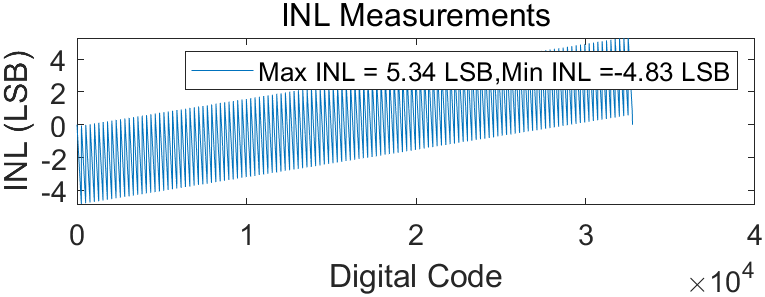
\includegraphics[width=0.7\textwidth]{pic/Co/INL2.png}
			\caption{第二级寄生电容的INL}
		\end{figure}

		\item \textbf{电阻热噪声} 测量T=300k时的电阻热噪声
		
		可以看到最差DNL为1LSB,最差INL为2.1LSB,SNR为85.82dB,SNDR为85.82dB,SFDR为137.49dB,THD为145.29dB,ENOB为13.96bit。

		DNL出现大量的不规则波动,,没有明显的轮廓了,符合噪声带来的影响。最后一位出现了失码。DFT图中看不出明显失真。
		\begin{figure}[H]
			\centering
			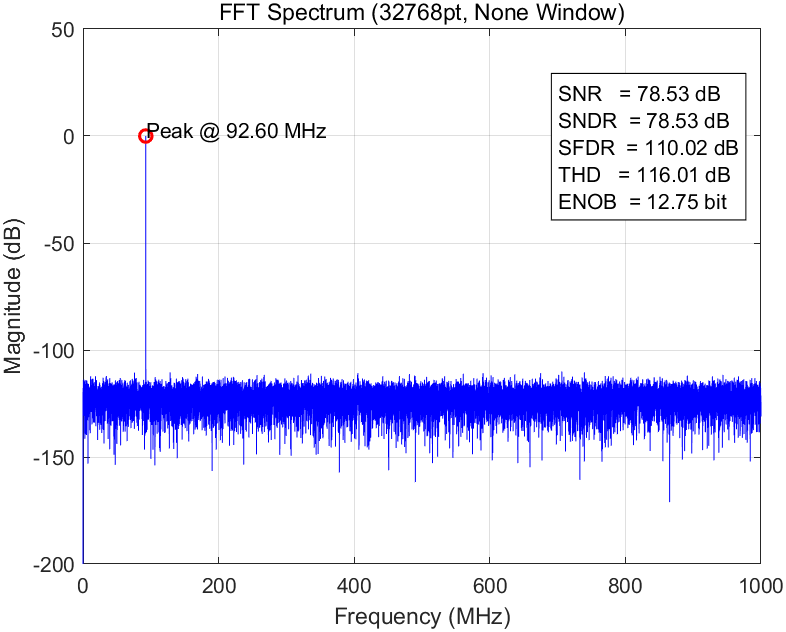
\includegraphics[width=0.7\textwidth]{pic/KT/DFT.png}
			\caption{电阻热噪声的动态特性} 
		\end{figure}

		\begin{figure}[H]
			\centering
			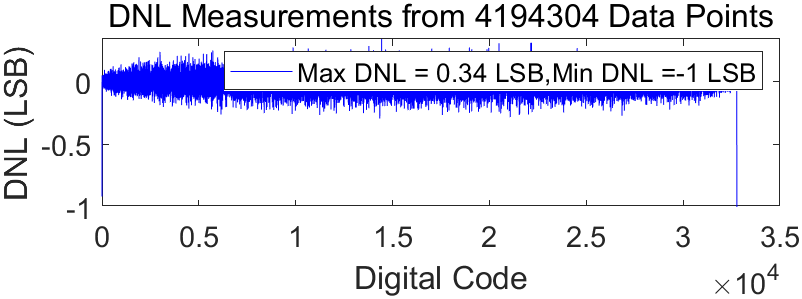
\includegraphics[width=0.7\textwidth]{pic/KT/DNL.png}
			\caption{电阻热噪声的DNL} 
		\end{figure}

		\begin{figure}[H]
			\centering
			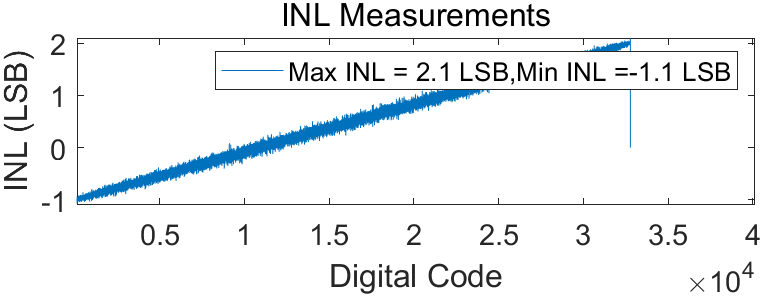
\includegraphics[width=0.7\textwidth]{pic/KT/INL.png}
			\caption{电阻热噪声的INL} 
		\end{figure}
	\end{itemize}


\subsubsection{所有非理想叠加}

	\begin{itemize}

	\item \textbf{电阻热噪声} 测量T=300k时的电阻热噪声
		
		可以看到最差DNL为1LSB,最差INL为2.1LSB,SNR为85.82dB,SNDR为85.82dB,SFDR为137.49dB,THD为145.29dB,ENOB为13.96bit。

		DNL出现大量的不规则波动,没有理想时明显的轮廓了,符合噪声带来的影响。最后一位出现了失码。DFT图中看不出明显失真。
		\begin{figure}[H]
			\centering
			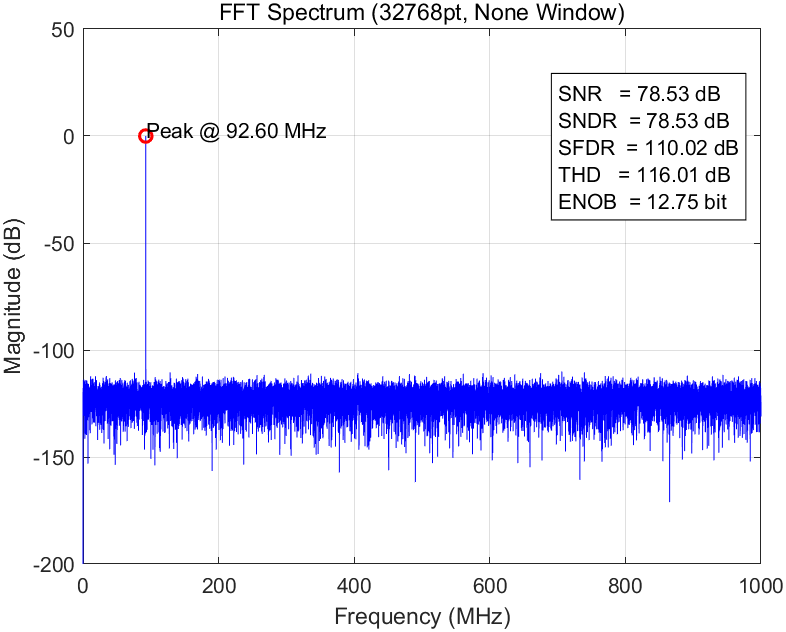
\includegraphics[width=0.7\textwidth]{pic/KT/DFT.png}
			\caption{电阻热噪声的动态特性} 
		\end{figure}

		\begin{figure}[H]
			\centering
			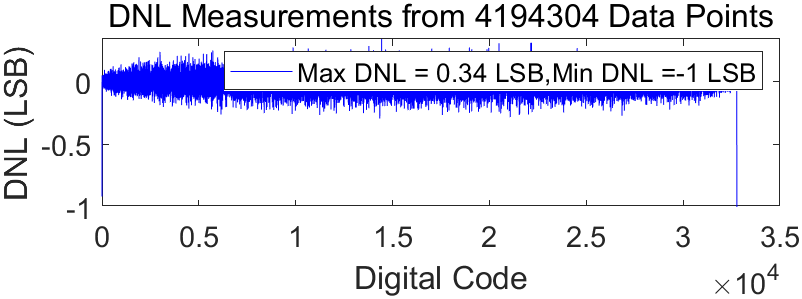
\includegraphics[width=0.7\textwidth]{pic/KT/DNL.png}
			\caption{电阻热噪声的DNL} 
		\end{figure}

		\begin{figure}[H]
			\centering
			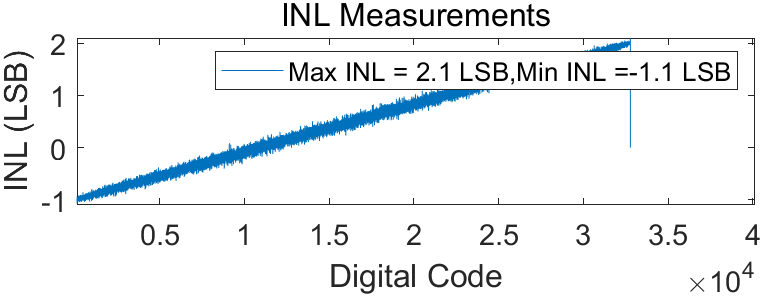
\includegraphics[width=0.7\textwidth]{pic/KT/INL.png}
			\caption{电阻热噪声的INL} 
		\end{figure}

	\item \textbf{时钟抖动} 测量jitter=100ps时的情况
		
		可以看到最差DNL为0.289LSB,最差INL为0.194LSB,SNR为89.66dB,SNDR为89.66dB,SFDR为132.16dB,THD为150.77dB,ENOB为14.6bit。

		DNL出现大量的不规则波动,没有理想时明显的轮廓了,符合时钟抖动带来的类似噪声的影响。DFT图中看不出明显失真。
		\begin{figure}[H]
			\centering
			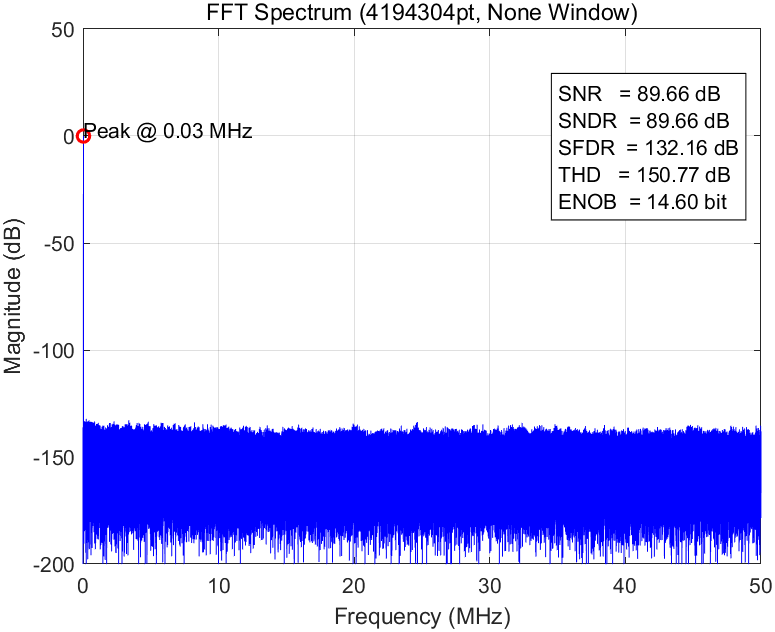
\includegraphics[width=0.7\textwidth]{pic/jitter/DFT.png}
			\caption{存在时钟抖动的动态特性} 
		\end{figure}

		\begin{figure}[H]
			\centering
			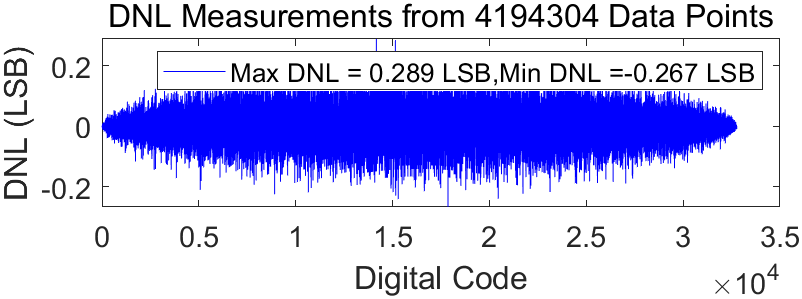
\includegraphics[width=0.7\textwidth]{pic/jitter/DNL.png}
			\caption{存在时钟抖动的DNL} 
		\end{figure}

		\begin{figure}[H]
			\centering
			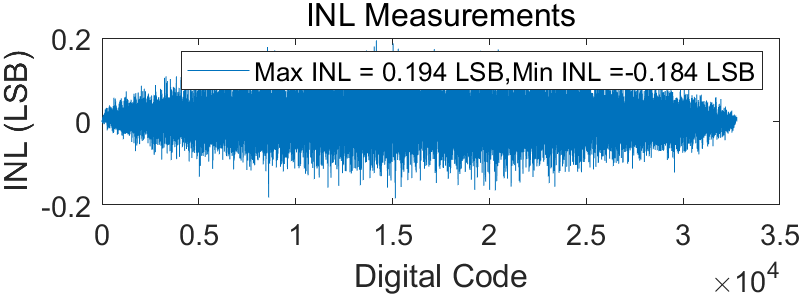
\includegraphics[width=0.7\textwidth]{pic/jitter/INL.png}
			\caption{存在时钟抖动的INL} 
		\end{figure}
    \end{itemize}

\subsubsection{所有非理想叠加}
$Mis_{OS} = 0.5 * LSB * randn()$;

$Mis_{Gain} = 1 + 0.2 * randn()$;

$Mis_{Clk} = 0.05 * 1/fs * randn()$;

实际级间增益为63.59;

带宽设置为为$0.1GHz$;

运放失调调为0.001V;

比较器失调调为0.005V;

第一级的寄生电容调为$Cp_{p1}  = 5fF $、$ Cp_{n1} = 5fF;$ 

第二级的寄生电容调为$Cp_{p2}  = 5fF $、$ Cp_{n2} = 5fF;$ 

T=300k时的电阻热噪声。

jitter=100ps。
		\begin{figure}[H]
			\centering
			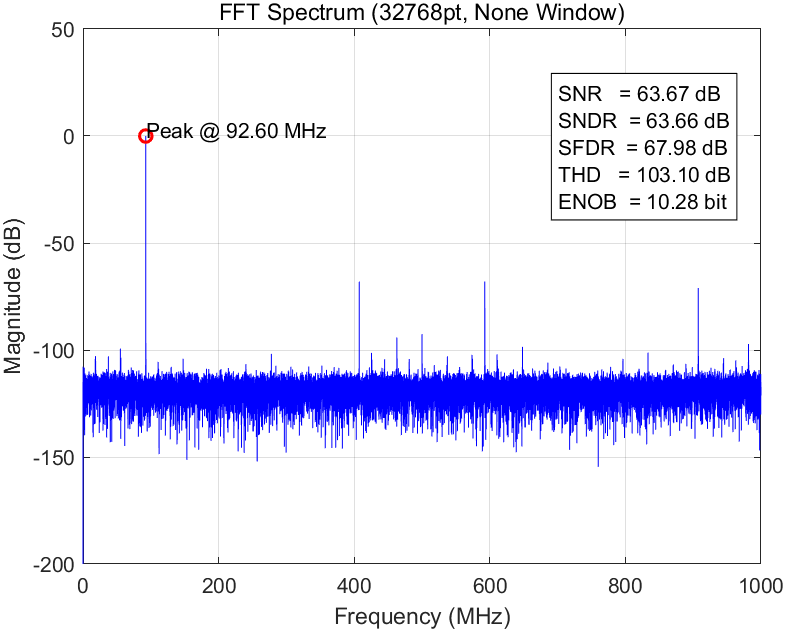
\includegraphics[width=0.7\textwidth]{pic/noideal/DFT.png}
			\caption{全都非理想时的动态特性} 
		\end{figure}

		\begin{figure}[H]
			\centering
			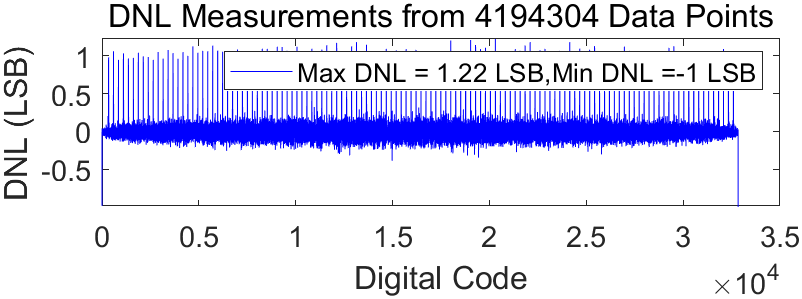
\includegraphics[width=0.7\textwidth]{pic/noideal/DNL.png}
			\caption{全都非理想时的DNL} 
		\end{figure}

		\begin{figure}[H]
			\centering
			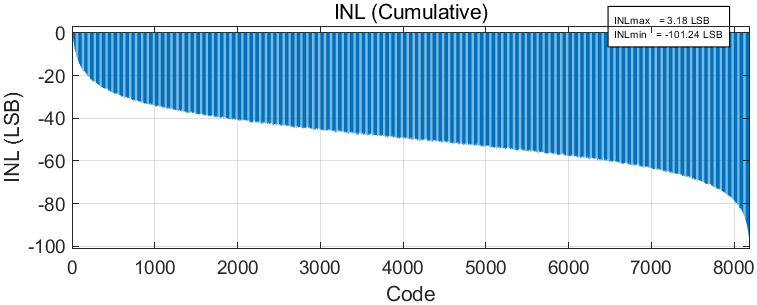
\includegraphics[width=0.7\textwidth]{pic/noideal/INL.png}
			\caption{全都非理想时的INL} 
		\end{figure}
		


		\begin{table}[H]
			\caption{静态/动态参数指标统计}
			\resizebox{\linewidth}{!}{
			\begin{tabular}{|c|c|c|c|c|c|c|c|}
				\hline
				\textbf{}        & \textbf{DNL(LSB)} & \textbf{INL(LSB)} & \textbf{SNR(dB)} & \textbf{SDNR(dB)} & \textbf{SFDR(dB)} & \textbf{THD(dB)} & \textbf{ENOB(bit)} \\ \hline
				\textbf{理想}      & 0.0303            & 0.0248            & 92.06            & 92.06             & 124.22            & 158.68           & 15                 \\ \hline
				\textbf{通道间失调失配} & 0.814            & 0.814            & 91.15            & 91.15             & 98.33            & 146.65           & 14.85             \\ \hline
				\textbf{通道间增益失配} & 0.989            & 1.07            & 91.4            & 91.4             & 101.82             & 145.5            & 14.89              \\ \hline
				\textbf{通道间时钟偏差} & 0.0222            & 0.0235            & 79.98            & 79.98             & 84.98             & 149.21           & 12.99               \\ \hline
				\textbf{级间增益误差}  & 0.832            & 1.62            & 86.35            & 86.35            & 104.63             & 159.92            & 14.05              \\ \hline
				\textbf{建立误差}    & 0.419           & 0.264          & 90.15            & 90.15            & 108.8          & 160.71             & 14.68            \\ \hline
				\textbf{运放失调}    & 0.866          & 0.866          & 92.06           & 92.06            & 126.88        & 161.51           & 15              \\ \hline
				\textbf{比较器失调}   & 0.719           & 0.719            & 92.07            & 92.07              & 124.89           & 160.76          & 15             \\ \hline
				\textbf{第一级寄生电容} & 0.0284            & 0.0259            & 92.07           & 92.07            & 124.48           & 154.85          & 15                \\ \hline
				\textbf{第二级寄生电容} & 0.994         & 5.34           & 77.81            & 77.81             & 94.75             & 157.67            & 12.63             \\ \hline
				\textbf{电阻热噪声}   & 1          & 2.1          & 85.82          & 85.82            & 137.49           & 145.29           & 13.96              \\ \hline
				\textbf{时钟抖动}   & 0.289          & 0.194          & 89.66          & 89.66            & 132.16           & 150.77           & 14.6              \\ \hline
				\textbf{上述非线性叠加} & 1.22          & 5.46        & 75.95            & 75.95             & 80.16            & 141.78           & 12.32             \\ \hline
			\end{tabular}
			}
		\end{table}
		
		结上表可以看到,但从ENOB进行分析,则通道间时钟偏差与第二级寄生电容对ENOB的有较大影响,其余的非理想因素影响较小。因此之后对Time Skew进行校正。

		冗余的存在能很好地抑制前一级的非理想性以及比较器、运放失调,与理论相符!

		电容寄生以及通道间的失配对失真的影响非常明显,SFDR明显下降。

		从DNL、INL图中可以看出,有限增益、有限带宽、电阻热噪声、时钟抖动对DNL、INL影响较大。
\newpage
		\section{Timing skew 校正}
		\subsection{时间校正方法一}
		\noindent
		本节,我们对 TI-ADC 各通道的采样时钟偏差(timing skew)进行校正,减小其对 SNR、SNDR、SFDR 的影响,提高 ENOB。
		
		\noindent
		\textbf{校正方法:}基于均值绝对差的后台校正
		
		\subsubsection{校正原理}
		
		\noindent
		考虑如\ref{fig:ti1}图所示信号,以两通道为例说明:
		\begin{figure}[H]
			\centering
			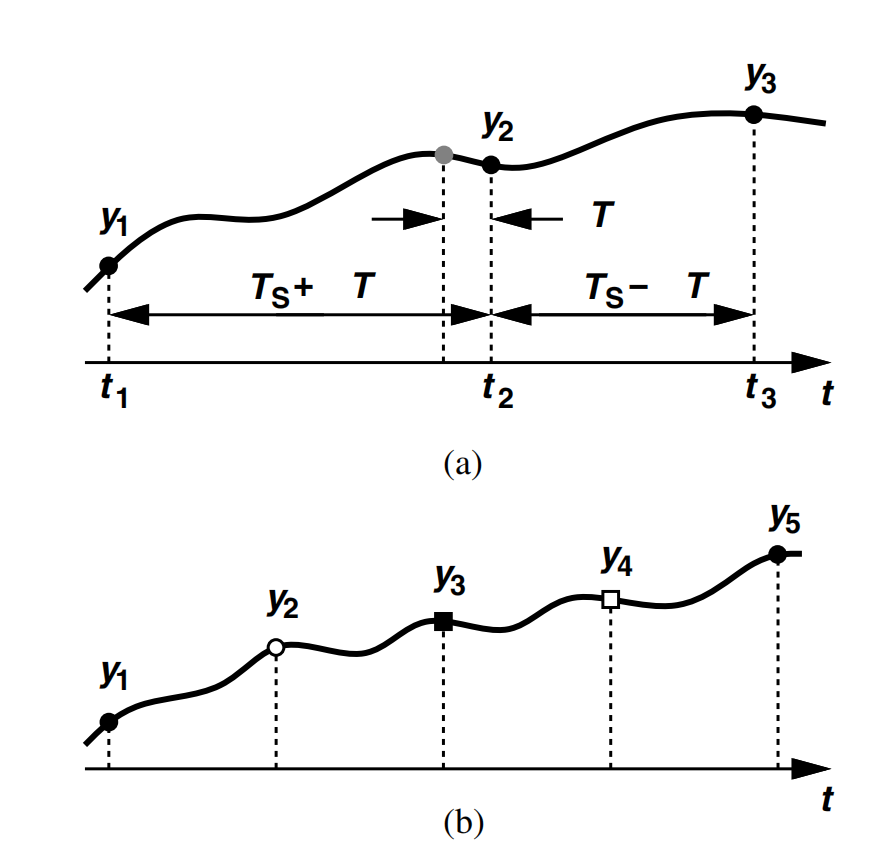
\includegraphics[width=0.7\textwidth]{figure/ti1.png}
			\caption{时间偏差校正原理图} \label{fig:ti1}
		\end{figure}
		
		
		设 $t_1$, $t_3$ 为通道1相邻采样时刻,不考虑时钟jitter,$t_3$比$t_1$延迟2$T_s$,$T_s=\frac{1}{f
		_s}$,(两通道TI-ADC,子ADC采样周期$T_{sub}=2*T_s$)$t_2$ 为通道2采样时刻,考虑通道2存在timing skew,不妨设延迟时间$T$。则$t_1$与$t_2$的时间间隔为$T_s+T$,$t_2$与$t_3$的时间间隔为$T_s-T$,即:
		
		\[
		t_2 = t_1 + T_s + T,\quad t_3 = t_2 + T_s - T
		\]
		
		采样值为 $y_1 = y(t_1)$,$y_2 = y(t_2)$,$y_3 = y(t_3)$,考虑以下式子:
		\begin{equation}
			\begin{aligned}
				E\left[\left(y_2-y_1\right)^2\right] & =E\left[y_2^2\right]+E\left[y_1^2\right]-2 E\left[y_2 y_1\right] \\
				& =\sigma_{y 2}^2+\sigma_{y 1}^2-2 E\left[y\left(t_1+T_S+T\right) y\left(t_1\right)\right]
			\end{aligned}
		\end{equation}
		
		在均方作用下,$\sigma_{y 1}^2=\sigma_{y 2}^2=\sigma_{y}^2$,因此
		\begin{equation}
			\begin{aligned}
				&E\left[\left(y_2-y_1\right)^2\right]=2 \sigma_y^2-2 E\left(y(t_1+T_S+T) \cdot y(t_1) \right) .\\
				&E\left[\left(y_3-y_2\right)^2\right]=2 \sigma_y^2-2 E\left(y(t_2+T_S-T) \cdot y(t_2)\right)
			\end{aligned}
		\end{equation}
		
		考虑信号y的自相关函数:
		$R(\tau)=E[y(t) \cdot y(t+\tau)]$
		
		则有,
		\begin{align*}
			E[(y_2 - y_1)^2] &= 2\sigma_y^2 - 2R(T_s + T) \\
			E[(y_3 - y_2)^2] &= 2\sigma_y^2 - 2R(T_s - T)
		\end{align*}
		\begin{align*}
			\Rightarrow E[(y_2 - y_1)^2] - \mathbb{E}[(y_3 - y_2)^2] = 2\left[ R(T_s - T) - R(T_s + T) \right]
		\end{align*}
		
		
		
		由于timing skew 的大小 $T$ 相对于ADC的周期 $T_s$ 是小量,泰勒展开得:
		\[
		E[(y_2 - y_1)^2] - E[(y_3 - y_2)^2] = -4T \dfrac{d R}{d \tau}
		\]
		
		由 Wiener–Khinchin 定理,一个平稳随机信号的自相关函数是它功率谱密度的反傅里叶变换,即
		\[
		R(\tau) = \int_{-\infty}^{\infty}   S(f) e^{j2\pi f\tau} df
		\]
		
		因此,我们可以求出自相关函数的导数:
		
		$$
		\begin{gathered}
			R^{\prime}(\tau)=\frac{d R}{d \tau}=\int_{-\infty}^{+\infty} j 2 \pi f S(f) \mathrm{e}^{j 2 \pi f \tau} \mathrm{df} \\
			=\int_{-\infty}^{+\infty} j 2 \pi f S(f)(\cos (2 \pi f \tau)+j \sin (2 \pi f \tau)) \mathrm{df}
		\end{gathered}
		$$
		
		
		已知对于实信号,功率谱密度是偶函数:
		
		$$
		\begin{gathered}
			S(f)=S(-f) \\
			R^{\prime}(\tau)=-\int_0^{+\infty} 4 \pi f S(f) \sin (2 \pi f \tau) d f
		\end{gathered}
		$$
		
		
		我们假设信号带宽限制在 Nyquist 采样频率之内,这也是一般满足的情况,进一步化简可得:
		
		$$
		R^{\prime}(T_s)=-\int_0^{T_s / 2} 4 \pi f S(f) \sin (2 \pi f T_s) df
		$$
		
		
		易知 $0<f<1 / 2 T s$ 时, $\sin (2 \pi f T s)>0$ .则 $R^{\prime}(\tau)<0$ ,这说明,当信号频率 fs 限制在奈奎斯特采样频率内时,其自相关函数的导数一定小于零。
		
		因此我们可以通过信号相邻通道的平方差均值求出时钟偏差的方向:
		
		$$
		\begin{aligned}
			& E\left[\left(\mathrm{y}_2-\mathrm{y}_1\right)^2\right]-E\left[\left(\mathrm{y}_3-\mathrm{y}_2\right)^2\right]=-4 \mathrm{~T} \frac{d R}{d \tau},   \frac{d R}{d \tau}<0 \\
			&\operatorname{sign}\left(E\left[\left(\mathrm{y}_2-\mathrm{y}_1\right)^2\right]-E\left[\left(\mathrm{y}_3-\mathrm{y}_2\right)^2\right]\right)=\operatorname{sign}(\mathrm{T})
		\end{aligned}
		$$
		
		
		同样的方法可以证明,利用相邻通道的绝对值差均值也是可以直接提取出 skew 方向的,考虑电路实现的复杂性,我们采样均值绝对差(MAD)的方法进行校正:
		
		在通道 2 上设置可调的延时单元,延时大小为 delay(注意:通道 1 是基准通道,不需要校正)
		
		\noindent
		计算相邻样本差,可通过加法器实现:
		
		$$
		\begin{gathered}
			y_1=y(t), \quad y_2=y(t+T s+\Delta t), \quad y_3=y(t_1+T s-\Delta t) \\
			y_{21}=\left|y_2-y_1\right|, \quad y_{32}=\left|y_3-y_2\right|
		\end{gathered}
		$$
		
		\noindent
		求均值,得到偏差方向,可通过均值滤波器实现:
		\[
		\text{sign}(E[(y_{21} - y_{32})^2] = \text{sign}(\Delta t)
		\]
		
		若 $\Delta t>0$ ,则将结果反馈到延时单元上,令 delay 增加一个负延时 $-t_0$ ;相反若 $\Delta t<0$ ,令 delay 增加一个正延时 $+t_0$
		
		重复上述步骤,进行迭代,最终 delay 会收敛于-$\Delta \mathrm{t}$ ,补偿时钟偏差的影响,得到精确的采样时刻
		
		\subsubsection{四通道校正}
		接下来分析四通道的情况,参考图\ref{fig:ti1}

		实现校正需要五个样本,分别为四个通道的样本( $\mathrm{y}_{1-4}$ )和通道 1 延迟一个周期的样本 $\left(\mathrm{y}_5\right)$ ,此时校正需要分两阶段进行:
		
		第一阶段:通过 $y_1, y_3, y_5$ 对通道 3 进行校正,方法和两通道情况一致。
		
		第二阶段:通道 3 已校正完毕,此时可将 $\mathrm{t}_3$ 视为精确的采样时刻, $\mathrm{t}_{31}=\mathrm{t}_{53}=2 \mathrm{Ts}$ ,则可重复之前的方法,对通道 2 和通道 4 进行校正
		
		电路结构示意图如下:
		\begin{figure}[H]
			\centering
			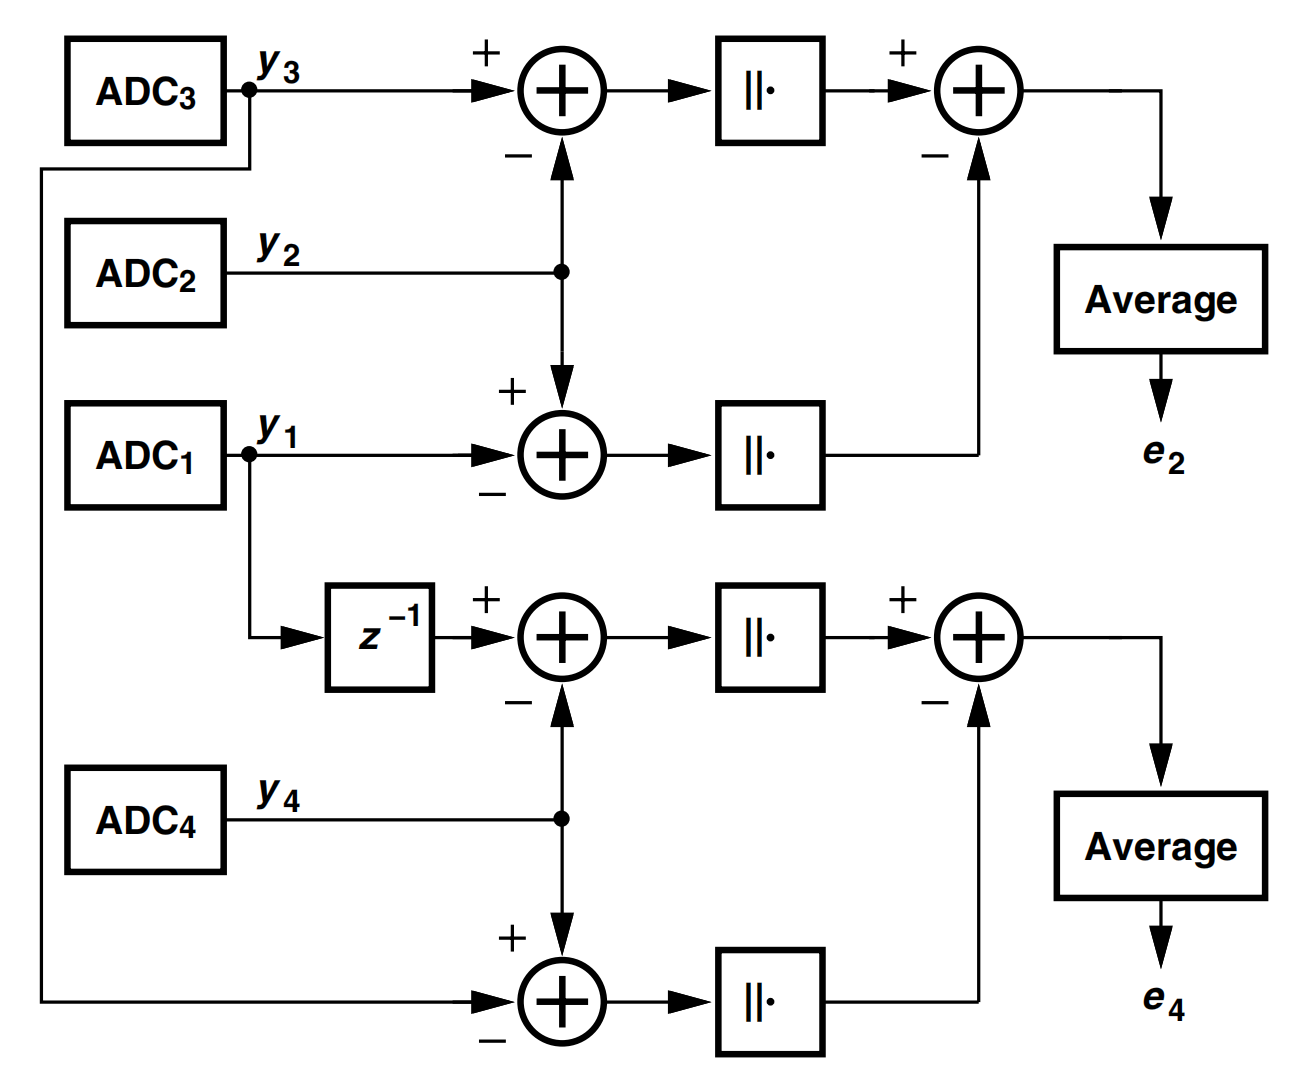
\includegraphics[width=0.7\textwidth]{figure/ti2.png}
			\caption{四通道ADC时间校正电路} \label{fig:ti2}
		\end{figure}
		
		\subsubsection{MATLAB 实现代码(节选)}
		

\begin{flushleft}
		\begin{lstlisting}[language=Matlab]
delay = zeros(1, n_ch);
t0 = (0.01 * 1/fs) / 100;
Vout_chs = zeros(n_ch + 1, floor(num/n_ch));
			Vout_diff = zeros(2, floor(num/n_ch));
sign_delta = zeros(1, n_ch);
iteration = 300;
alpha0 = 1;
beta = 0;
delay_err_log = zeros(iteration, n_ch);

for k = 1 : iteration
...
if k < iteration / 2
Vout_diff(1,:) = abs(Vout_chs(1,:) - Vout_chs(3,:));
Vout_diff(2,:) = abs(Vout_chs(3,:) - Vout_chs(5,:));
sign_delta(3) = -sign(sum(Vout_diff(1,:) - Vout_diff(2,:)));
elseif k == iteration / 2
sign_delta(3) = 0;
else
Vout_diff(1,:) = abs(Vout_chs(1,:) - Vout_chs(2,:));
Vout_diff(2,:) = abs(Vout_chs(2,:) - Vout_chs(3,:));
sign_delta(2) = -sign(sum(Vout_diff(1,:) - Vout_diff(2,:)));
Vout_diff(1,:) = abs(Vout_chs(3,:) - Vout_chs(4,:));
Vout_diff(2,:) = abs(Vout_chs(4,:) - Vout_chs(5,:));
sign_delta(4) = -sign(sum(Vout_diff(1,:) - Vout_diff(2,:)));
end

alpha = alpha0 / (1 + beta*k);
delay = delay + alpha * t0 * sign_delta;
...
end
		\end{lstlisting}
\end{flushleft}

		
		\subsubsection{校正效果分析}
		\begin{itemize}
			\item 
		\textbf{\underline{固定 skew 情况:}}
		
		设定 timing skew 为:
		
		\[
		\text{Mis\_TS} = 0.005 \times \frac{1}{f_s} \times [-0.2, 0.4, 0.3, -0.6]
		\]
		
		没有校正时,静态分析和动态分析结果如下图:
		\begin{figure}[H]
			\centering
			\begin{minipage}{0.49\linewidth}
				\centering
				\includegraphics[width=0.9\linewidth]{figure/result1.png}
			\end{minipage}
			\begin{minipage}{0.49\linewidth}
				\centering
				\includegraphics[width=0.9\linewidth]{figure/result2.png}
			\end{minipage}
			\caption{未校正时静态和动态分析结果} 
			\label{fig:result12}
		\end{figure}
		
		
		加入校正后,静态和动态分析结果如图:
		\begin{figure}[H]
			\centering
			\begin{minipage}{0.49\linewidth}
				\centering
				\includegraphics[width=0.9\linewidth]{figure/result3.png}
			\end{minipage}
			\begin{minipage}{0.49\linewidth}
				\centering
				\includegraphics[width=0.9\linewidth]{figure/result4.png}
			\end{minipage}
			\caption{校正后静态和动态分析结果} 
			\label{fig:result34}
		\end{figure}
		
		各通道校正残差收敛情况如下:
		\begin{figure}[H]
			\centering
			\includegraphics[width=0.7\textwidth]{figure/result5.png}
			\caption{各通道残差收敛情况} 
			\label{fig:result5}
		\end{figure}
		
		
		可以看到,校正效果非常明显。
		
		\item
		\textbf{\underline{随机 skew 情况:}}
		timing skew 由如下语句随机生成:
		\[
		\text{Mis\_TS} = 0.005 \times \frac{1}{f_s} \times \text{randn}(1, n\_ch)
		\]
		
		\noindent 
		fs 为 100 MHz ,即 skew 均值为 0 ps 方差 50 ps 的正态分布
		下表统计了十次由随机数种子随机生成的 skew 校正前后的 ENOB 和 SNDR,其中设置迭代次数为 350 次,经检验能确保 $\pm 4 \sigma$ 情况均收敛:

        	\begin{table}[H]
        		\centering
        		\caption{校正情况指标统计}
        		\begin{tabular}{|l|l|l|l|}
        			\hline \multicolumn{2}{|c|}{校正前} & \multicolumn{2}{|c|}{校正后} \\
        			\hline ENOB(bit) & SNDR(dB) & ENOB(bit) & SNDR(dB) \\
        			\hline 9.03 & 58.23 & 12.99 & 79.96 \\
        			\hline 9.06 & 56.33 & 12.99 & 79.94 \\
        			\hline 10.28 & 63.61 & 12.97 & 79.86 \\
        			\hline 9.27 & 57.58 & 12.99 & 79.97 \\
        			\hline 8.73 & 54.29 & 12.99 & 79.98 \\
        			\hline 8.89 & 55.28 & 12.99 & 79.94 \\
        			\hline 9.77 & 60.55 & 12.99 & 79.99 \\
        			\hline 10.50 & 64.99 & 12.99 & 79.97 \\
        			\hline 10.04 & 62.22 & 12.98 & 79.90 \\
        			\hline 9.24 & 57.40 & 12.99 & 79.94 \\
        			\hline
        		\end{tabular}
        	\end{table}

		\end{itemize}
		
		\subsubsection{迭代次数分析}
		在不同迭代次数下,进行多次随机数生成 skew,并统计 ENOB 和 SNDR 的平均值。

		\begin{figure}[H]
			\centering
			\includegraphics[width=0.7\textwidth]{figure/result6.png}
			\caption{SNDR/ENOB随迭代次数变化} 
			\label{fig:result6}
		\end{figure}
		
		可以看到,在统计条件下,校正对 ENOB 和 SNDR 的改善非常明显,且大约 300 次迭
		代就能实现大部分情况的收敛,ENOB 和 SNDR 达到最大。
		
		
		\subsection{时间校正方法二:基于自相关函数的校正}
		
		\subsubsection{校正原理}
		
		\noindent
		首先计算所有相邻通道的自相关函数,包括最后一个通道与第一个通道的下一次采样的自相关。可以通过乘法器和均值滤波器实现,即:
		\begin{equation}
			\mathbb{E}\left(x_i[k] x_{i+1}[k]\right)=R\left(t_{i, i+1}\right)
		\end{equation}
		
		以四通道为例,求出$R\left(t_{1.2}\right)$,$R\left(t_{2,3}\right)$,$R\left(t_{3,4}\right)$和$$R\left(t_{4,1}\right)$$.
		
		理想采样时刻,有$t_{1,2}=t_{2,3}=t_{3,4}=t_{4,1}=T_s$,存在时钟偏差时,考虑偏差相对采样周期是极小量,由泰勒展开易得:
		
		\begin{equation}
			\begin{aligned}
				& \left(R\left(t_{1,2}\right)+R\left(t_{2,3}\right)+R\left(t_{3,4}\right)+R\left(t_{4,1}\right)\right) / 4 \\
				\approx & R\left(T_s\right)+R^{\prime}\left(T_s\right)\left(t_{1,2}+t_{2,3}+t_{3,4}+t_{4,1}-4 T_s\right) / 4 \\
				= & R\left(T_s\right)
			\end{aligned}
		\end{equation}
		
		上式表面,$R(T_s)$可以通过对四个相关函数求平均来逼近。
		
		我们再考虑,自相关函数在数个Ts范围内近似线性,则可以认为,$R(k T_s)≈kR(T_s)$。下图为四通道TI-ADC的采样时刻图,白色表示理想采样时刻,红色表示实际采样时刻,采样时刻可以通过自相关函数来提取。
		
		\begin{figure}[H]
			\centering
			\includegraphics[width=0.7\textwidth]{figure/cor1.png}
			\caption{时间偏差校正原理图} \label{fig:cor1}
		\end{figure}
		
		由泰勒展开,我们可以通过如下式子进一步提取出所有通道的采样时刻偏差:
		\begin{equation}
			\begin{aligned}
				\Delta R_4 & =R\left(t_{1,2}\right)+R\left(t_{2,3}\right)+R\left(t_{3,4}\right)-3 R\left(T_s\right) \\
				& \approx R^{\prime}\left(T_s\right) \Delta t_4 .
			\end{aligned}
		\end{equation}
		
		\begin{equation}
			\begin{aligned}
				\Delta R_3 & =R\left(t_{1,2}\right)+R\left(t_{2,3}\right)-2 R\left(T_s\right) \\
				& \approx R^{\prime}\left(T_s\right)\left(t_{1,2}+t_{2,3}-2 T_s\right) \\
				& =R^{\prime}\left(T_s\right) \Delta t_3 .
			\end{aligned}
		\end{equation}
		
		\begin{equation}
			\Delta R_2=R\left(t_{1,2}\right)-R\left(T_s\right) \approx R^{\prime}\left(T_s\right) \Delta t_2
		\end{equation}
		
		前文我们已经证明 $R^{\prime}(T_s)<0$ ,因此可以通过 $\Delta R_i$ 的符号来求出 $\Delta t_i$ 的符号,进而确定反馈极性。

			
		\subsubsection{MATLAB 实现代码}
		接下来通过代码来解释校正步骤:
		
		\begin{flushleft}
			\begin{lstlisting}[language=Matlab]
for i= 1:n_ch
……(ADC采样+量化)
% 各通道得到的样本
Vout_chs(i,:) = D .* Vref / 2^N;
end
% 求出相邻通道的自相关函数
for i =1:n_ch
if i<n_ch
R_ti(i) = sum( Vout_chs(i,1:M-1) .* Vout_chs(i+1,1:M-1) ) / (M-1);
else
R_ti(i) = sum( Vout_chs(n_ch,1:M-1) .* Vout_chs(1,2:M) ) / (M-1);
end
end
% calculate calibration orientation 
% 计算R(Ts)的近似值
R_ts = sum(R_ti, "all")/n_ch;
% 求出ΔR,进而求出反馈极性
for i=1:n_ch
R_delta(i) = sum(R_ti(1:i-1)) - (i-1)*R_ts;
end
sign_delta = sign(R_delta);
% 反馈,迭代求解
alpha = alpha0 / (1 + beta*k);
delay = delay + alpha*t0*sign_delta .* ones(1,n_ch);
for i = 1:n_ch
delay_err_log(k, i) = delay(i) + Mis_TS(i) - Mis_TS(1);
end
			\end{lstlisting}
		\end{flushleft}
		
	我们可以发现,该方法的优点是可以同时对所有通道进行校正。
		
		
		\subsubsection{校正结果}
		
		考虑 timing skew 由如下语句随机生成:
		
		\[
		\text{Mis\_TS} = 0.005 \times \frac{1}{f_s} \times \text{randn}(1, n\_ch)
		\]

		
		fs 为 100 MHz ,即 skew 均值为 0 ps 方差 50 ps 的正态分布下表统计了十次由随机数种子随机生成的 skew 校正前后的 ENOB 和 SNDR,其中设置迭代次数为 200 次,经检验能确保 $\pm 4 \sigma$ 情况均收敛:
		
		
		
		
		\begin{table}[H]
			\centering
			\caption{校正情况指标统计}
			\begin{tabular}{|l|l|l|l|}
				\hline \multicolumn{2}{|c|}{校正前} & \multicolumn{2}{|c|}{校正后} \\
				\hline ENOB(bit) & SNDR(dB) & ENOB(bit) & SNDR(dB) \\
				\hline 9.03 & 58.23 & 11.47 & 70.83 \\
				\hline 9.06 & 56.33 & 11.50 & 71.02 \\
				\hline 10.28 & 63.61 & 11.53 & 71.16 \\
				\hline 9.27 & 57.58 & 11.54 & 71.24 \\
				\hline 8.73 & 54.29 & 11.48 & 70.84 \\
				\hline 8.89 & 55.28 & 11.47 & 70.82 \\
				\hline 9.77 & 60.55 & 11.51 & 71.05 \\
				\hline 10.50 & 64.99 & 11.50 & 70.96 \\
				\hline 10.04 & 62.22 & 11.54 & 71.21 \\
				\hline 9.24 & 57.40 & 11.48 & 70.88 \\
				\hline
			\end{tabular}
		\end{table}
		

		
		
		
		
		某一次校正的残差收敛曲线和动态/静态分析结果如图\ref{fig:cor2}和\ref{fig:cor34}:
		\begin{figure}[H]
			\centering
			\includegraphics[width=0.7\textwidth]{figure/cor2.png}
			\caption{方法二时间校正残差收敛曲线} \label{fig:cor2}
		\end{figure}
		
		
		
			\begin{figure}[H]
				\centering
				\begin{minipage}{0.49\linewidth}
					\centering
					\includegraphics[width=0.9\linewidth]{figure/cor3.png}
				\end{minipage}
				\begin{minipage}{0.49\linewidth}
					\centering
					\includegraphics[width=0.9\linewidth]{figure/cor4.png}
				\end{minipage}
				\caption{方法二时间校正动态/静态分析结果} 
				\label{fig:cor34}
			\end{figure}
			
		可以发现,该方法修正精度不如方法一,因为收玫的位置存在误差。推测原因包括:
		
		1. $\mathrm{R}(\mathrm{Ts})$ 使用对所有自相关函数求平均的方式近似计算,存在误差(次要)
		
		2.$\Delta R$ 的计算需要自相关函数是线性,相当于 $T s$ 尺度下的泰勒展开一阶放缩,误差较大 (主要)
			
		
		\subsubsection{迭代次数分析}
		在不同迭代次数下,进行多次随机数生成 skew,并统计 ENOB 和 SNDR 的平均值。
		
		\begin{figure}[H]
			\centering
			\includegraphics[width=0.7\textwidth]{figure/cor6.png}
			\caption{SNDR/ENOB随迭代次数变化} 
			\label{fig:cor6}
		\end{figure}
		
		\underline{可以看到,最佳迭代次数大概为150次,即只需要方法一所需时间的一半就能完成校正。}
\newpage
		\section{项目感想与需要注意的点}
		\subsection{时间校正方法的选取}
		时间偏差是影响TI-ADC精度的关键因素,相比增益误差和放大器失调的因素,采样时刻不属于统计量,无法通过求平均的方式进行消除,因此较难校正。
		通过对大量相关文献的查阅,我们发现目前时钟偏差校正方法可以通过其对偏差的提取方式划分为大致三种:
		\begin{itemize}
			\item 第一种方法是通过一个额外参考通道进行校正,令参考通道的采样时刻能与每一个子ADC的采样时刻对齐,然后通过数字域上自相关函数等方法求出参考通道与每个通道的采样样本偏差值,最后对偏差值进行纠正。例如,文献\cite{ref1}在原有TI-ADC上增加了一个单比特单通道的参考ADC,并令其采样时刻覆盖子ADC采样时刻,并求出参考ADC样本相对各通道样本的相关函数,利用LSM算法和反馈到各通道的延时线对其极大值进行迭代逼近。该方法涉及额外ADC的使用,且需要确保该参考ADC的采样时刻是精确的。
			
			\item 第二种方法需要一个额外的信号发生器生成一组参考信号,并将其送入每个通道中进行额外的采样,通过采样结果可以检测各通道的时钟偏差情况。例如文献\cite{ref2}使用过零点检测的方法,当周期性参考信号与采样时钟不同步时,相邻两个采样器之间出现过零点的概率与它们之间的采样时间间隔成正比,由此可以反应时钟偏差的极性。该方法需要增加高精度的信号发生器,且每个通道需要额外进行一次采样。
			
			\item 第三种方法是基于输入信号的统计特性来提取时钟误差,通过对比不同通道间采样值的相关性进行检测。在检测出极性之后,可以通过调节采样时刻在模拟域中进行校正,同时也可以利用数字滤波器在数字域中进行校正。
			
			相比于前两类校准技术,第三类方法最显著的优势在于:\textbf{无需模拟硬件开销,所有的校准可以完全在数字域中完成},因此本次仿真选择第三种。
			
		\end{itemize}
		
		\subsection{项目过程中需要注意的点}
		\begin{itemize}
			\item 流水线中后一级ADC与前一级不同,前一级的sub ADC直接完成N1次比较与作差,后一级的sub ADC进行N2次比较,但是只需要进行N2-1次作差。
			
			\item 测量DNL时使用sin进行测量受挫。使用sin函数进行测量时,由于测量数量不是无限多,可以得到近似正确的DNL,实际仍有些许偏差。但由于sin的pdf不同,在除以每个码的理想值后,相当于对DNL的偏差进行了加权,从而导致INL在测量点数不够多的情况下偏差很大。
			
			\item 将矩阵的维度设置错误,从而导致电脑内存不足,无法进行特别多的采样,导致误差很大。之后改正了维度错误,正常运行。
			
			\item 计算自相关函数的硬件开销过大,使用绝对值差函数进行替换:
			由于计算自相关函数需要对庞大的样本进行乘积,硬件开销过于巨大,我们推测实际布置电路时不具备可行性,因此考虑其替代方案。文献[8]指出,均值绝对差(MAD,Mean Absolute Deviation)可用于替代相关性计算,在一般情况下很难证明二者的等价性,此处以正弦输入信号 $V(t)=\cos (\omega t) V(t)$ 为例进行分析。
			
			设采样间隔为 $\tau$ ,则两采样值间的 MAD 可表示为:
			
			$$
			\operatorname{MAD}(\tau)=|\cos (\omega t)-\cos (\omega(t+\tau))|=2 \cdot\left|\sin \left(\frac{\omega \tau}{2}\right) \cdot \sin \left(\omega t+\frac{\omega \tau}{2}\right)\right|
			$$
			
			
			当采样相位均匀分布时,第二项 $\sin (\omega t+\omega \tau / 2)$ 的期望值趋近于 $2 / \pi$ ,从而有:
			
			$$
			\operatorname{MAD}(\tau)=\frac{4}{\pi} \cdot\left|\sin \left(\frac{\omega \tau}{2}\right)\right|
			$$
			
			
			比较正弦函数的自相关函数 $R(\tau)=\cos (\omega \tau)$ 的波形。显然MAD( $\tau$ )与 $R(\tau)$ 的单调性恰好相反:
			
			\begin{figure}[H]
				\centering
				\includegraphics[width=0.7\textwidth]{figure/feeling1.png}
				\caption{自相关和MAD的比较} 
				\label{fig:feeling1}
			\end{figure}
			
			通过这两个特殊情况,我们可推断出:MAD′(Ts​) 与 R′(Ts​) 的符号总是相反的。因此,MAD与自相关函数在提取时序偏差误差方面具有等效性。
			
			然而,使用均值绝对值就行校正的采样时刻必须处于两个精确的采样时刻之间,因此无法同时对多个存在偏差的通道进行校正。
			
			\item 关于多通道(>2)情况的校正
			
			基于自相关的校正方法存在如何提取 $\mathrm{R}(\mathrm{Ts})$ 的问题,理论上最精确的方法是使用同一通道的相邻两次采样(间隔一个 n_ch*Ts 的延时)进行提取。但该方法只能对一个通道 (即采样时刻位于中点处的那个通道)进行校正。在四通道的情况下,只能先对通道 3进行校正,随后再对 2 和 4 进行校正。我们也找到了能同时对所有通道进行校正的方法,例如文献\cite{ref3}(本次项目采用的校正方法2)使用近似 $\mathrm{R}\left(\mathrm{Ts}_s\right) \approx \sum_{i=1}^{n-c h} R\left(t_i, t_{i+1}\right)$ 来计算。并近似自相关函数 $\mathrm{R}(\tau)$ 在一个采样周期内是线性的,这样可以同时对所有通道进行修正:
			
			\begin{figure}[H]
				\centering
				\includegraphics[width=0.7\textwidth]{figure/feeling2.png}
				\caption{四通道时间校正方法示意图} 
				\label{fig:feeling2}
			\end{figure}
			
			然而,我们在实际建模中发现该方法校正结果误差较大,通道延时相对skew的残差往往无法收敛到足够小的位置,ENOB只能提升大于1.5-2.5bit,最大修正ENOB大约为11.5
			
			\item 校正精度和速度的权衡
			
			对于在数字域提取误差、在模拟域进行校正的时序偏差校正技术而言,最终的校准精度受数字模块和模拟模块的共同影响。其中,模拟精度主要体现在可调延迟线的调节步长上,更小的步长意味着更精确的收敛域,但也增加了需要的迭代次数;而数字精度的影响则更为复杂。直观来看,通过增加平均采样的数量可以提升数字域的精度;但与此同时,这也会导致收敛速度下降。而校正方法也是影响进度的关键因素。采用单次只校正一个通道的方法能确保最高的校正精度,但大大增加了迭代次数;而多通道同时校正的方法虽然存在更大的误差,却能确保一定的校正速度,且不容易随通道数的变化而改变。总的来说,数字校准系统存在一个根本性的权衡关系:即校准精度与收敛速度之间的矛盾。
			
		\end{itemize}
		
		
		
		
		
\clearpage

%============= 参考文献 =====================
\addcontentsline{toc}{section}{参考文献}
%\bibliography{bibfile}
\begin{thebibliography}{100}
\bibitem{ref1} M. El-Chammas and B. Murmann, “A 12-GS/s 81-mW 5-bit timeinterleaved flash ADC with background timing skew calibration,” IEEE J. Solid-State Circuits, vol. 46, no. 4, pp. 838–847, Apr. 2011.
\bibitem{ref2} C.-C. Huang, C.-Y. Wang, and J.-T. Wu, “A CMOS 6-bit 16-GS/s timeinterleaved ADC using digital background calibration techniques,” IEEE J. Solid-State Circuits, vol. 46, no. 4, pp. 848–858, Apr. 2011.
\bibitem{ref3} M. Gu, Y. Tao, X. He, Y. Zhong, L. Jie and N. Sun, "A 1-GS/s 11-b Time-Interleaved SAR ADC With Robust, Fast, and Accurate Autocorrelation-Based Background Timing-Skew Calibration," in IEEE Journal of Solid-State Circuits, vol. 60, no. 2, pp. 421-431, Feb. 2025, doi: 10.1109/JSSC.2024.3421363.
\bibitem{ref4} 本pj在原理介绍部分的部分图片来自江文宁老师和叶凡老师的ADDA课程课件。
\end{thebibliography}
\clearpage
%=============  致谢  ======================
% \include{body/acknowledge}
%\include{body/appendices}

\end{document}
%%%%%%%%%% 结束 %%%%%%%%%%